\documentclass[11pt,preprint]{elsarticle}

\usepackage{lmodern}
%%%% My spacing
\usepackage{setspace}
\setstretch{1.2}
\DeclareMathSizes{12}{14}{10}{10}

% Wrap around which gives all figures included the [H] command, or places it "here". This can be tedious to code in Rmarkdown.
\usepackage{float}
\let\origfigure\figure
\let\endorigfigure\endfigure
\renewenvironment{figure}[1][2] {
    \expandafter\origfigure\expandafter[H]
} {
    \endorigfigure
}

\let\origtable\table
\let\endorigtable\endtable
\renewenvironment{table}[1][2] {
    \expandafter\origtable\expandafter[H]
} {
    \endorigtable
}


\usepackage{ifxetex,ifluatex}
\usepackage{fixltx2e} % provides \textsubscript
\ifnum 0\ifxetex 1\fi\ifluatex 1\fi=0 % if pdftex
  \usepackage[T1]{fontenc}
  \usepackage[utf8]{inputenc}
\else % if luatex or xelatex
  \ifxetex
    \usepackage{mathspec}
    \usepackage{xltxtra,xunicode}
  \else
    \usepackage{fontspec}
  \fi
  \defaultfontfeatures{Mapping=tex-text,Scale=MatchLowercase}
  \newcommand{\euro}{€}
\fi

\usepackage{amssymb, amsmath, amsthm, amsfonts}

\def\bibsection{\section*{References}} %%% Make "References" appear before bibliography


\usepackage[numbers]{natbib}

\usepackage{longtable}
\usepackage[margin=2.3cm,bottom=2cm,top=2.5cm, includefoot]{geometry}
\usepackage{fancyhdr}
\usepackage[bottom, hang, flushmargin]{footmisc}
\usepackage{graphicx}
\numberwithin{equation}{section}
\numberwithin{figure}{section}
\numberwithin{table}{section}
\setlength{\parindent}{0cm}
\setlength{\parskip}{1.3ex plus 0.5ex minus 0.3ex}
\usepackage{textcomp}
\renewcommand{\headrulewidth}{0.2pt}
\renewcommand{\footrulewidth}{0.3pt}

\usepackage{array}
\newcolumntype{x}[1]{>{\centering\arraybackslash\hspace{0pt}}p{#1}}

%%%%  Remove the "preprint submitted to" part. Don't worry about this either, it just looks better without it:
\makeatletter
\def\ps@pprintTitle{%
  \let\@oddhead\@empty
  \let\@evenhead\@empty
  \let\@oddfoot\@empty
  \let\@evenfoot\@oddfoot
}
\makeatother

 \def\tightlist{} % This allows for subbullets!

\usepackage{hyperref}
\hypersetup{breaklinks=true,
            bookmarks=true,
            colorlinks=true,
            citecolor=blue,
            urlcolor=blue,
            linkcolor=blue,
            pdfborder={0 0 0}}


% The following packages allow huxtable to work:
\usepackage{siunitx}
\usepackage{multirow}
\usepackage{hhline}
\usepackage{calc}
\usepackage{tabularx}
\usepackage{booktabs}
\usepackage{caption}


\newenvironment{columns}[1][]{}{}

\newenvironment{column}[1]{\begin{minipage}{#1}\ignorespaces}{%
\end{minipage}
\ifhmode\unskip\fi
\aftergroup\useignorespacesandallpars}

\def\useignorespacesandallpars#1\ignorespaces\fi{%
#1\fi\ignorespacesandallpars}

\makeatletter
\def\ignorespacesandallpars{%
  \@ifnextchar\par
    {\expandafter\ignorespacesandallpars\@gobble}%
    {}%
}
\makeatother


% definitions for citeproc citations
\NewDocumentCommand\citeproctext{}{}
\NewDocumentCommand\citeproc{mm}{%
\href{\#cite.\detokenize{#1}}{#2}\nocite{#1}}

\makeatletter
% allow citations to break across lines
\let\@cite@ofmt\@firstofone
% avoid brackets around text for \cite:
\def\@biblabel#1{}
\def\@cite#1#2{{#1\if@tempswa , #2\fi}}
\makeatother
\newlength{\cslhangindent}
\setlength{\cslhangindent}{1.5em}
\newlength{\csllabelwidth}
\setlength{\csllabelwidth}{3em}
\newenvironment{CSLReferences}[2] % #1 hanging-indent, #2 entry-spacing
{\begin{list}{}{%
	\setlength{\itemindent}{0pt}
	\setlength{\leftmargin}{0pt}
	\setlength{\parsep}{0pt}
	% turn on hanging indent if param 1 is 1
	\ifodd #1
	\setlength{\leftmargin}{\cslhangindent}
	\setlength{\itemindent}{-1\cslhangindent}
	\fi
	% set entry spacing
	\setlength{\itemsep}{#2\baselineskip}}}
{\end{list}}

\usepackage{calc}
\newcommand{\CSLBlock}[1]{\hfill\break\parbox[t]{\linewidth}{\strut\ignorespaces#1\strut}}
\newcommand{\CSLLeftMargin}[1]{\parbox[t]{\csllabelwidth}{\strut#1\strut}}
\newcommand{\CSLRightInline}[1]{\parbox[t]{\linewidth - \csllabelwidth}{\strut#1\strut}}
\newcommand{\CSLIndent}[1]{\hspace{\cslhangindent}#1}


\urlstyle{same}  % don't use monospace font for urls
\setlength{\parindent}{0pt}
\setlength{\parskip}{6pt plus 2pt minus 1pt}
\setlength{\emergencystretch}{3em}  % prevent overfull lines
\setcounter{secnumdepth}{5}

%%% Use protect on footnotes to avoid problems with footnotes in titles
\let\rmarkdownfootnote\footnote%
\def\footnote{\protect\rmarkdownfootnote}
\IfFileExists{upquote.sty}{\usepackage{upquote}}{}

%%% Include extra packages specified by user
\usepackage{sectsty}
\sectionfont{\bfseries\large}
\subsectionfont{\bfseries\normalsize}\usepackage{booktabs}
\usepackage{longtable}
\usepackage{array}
\usepackage{multirow}
\usepackage{wrapfig}
\usepackage{float}
\usepackage{colortbl}
\usepackage{pdflscape}
\usepackage{tabu}
\usepackage{threeparttable}
\usepackage{threeparttablex}
\usepackage[normalem]{ulem}
\usepackage{makecell}
\usepackage{xcolor}

%%% Hard setting column skips for reports - this ensures greater consistency and control over the length settings in the document.
%% page layout
%% paragraphs
\setlength{\baselineskip}{12pt plus 0pt minus 0pt}
\setlength{\parskip}{12pt plus 0pt minus 0pt}
\setlength{\parindent}{0pt plus 0pt minus 0pt}
%% floats
\setlength{\floatsep}{12pt plus 0 pt minus 0pt}
\setlength{\textfloatsep}{20pt plus 0pt minus 0pt}
\setlength{\intextsep}{14pt plus 0pt minus 0pt}
\setlength{\dbltextfloatsep}{20pt plus 0pt minus 0pt}
\setlength{\dblfloatsep}{14pt plus 0pt minus 0pt}
%% maths
\setlength{\abovedisplayskip}{12pt plus 0pt minus 0pt}
\setlength{\belowdisplayskip}{12pt plus 0pt minus 0pt}
%% lists
\setlength{\topsep}{10pt plus 0pt minus 0pt}
\setlength{\partopsep}{3pt plus 0pt minus 0pt}
\setlength{\itemsep}{5pt plus 0pt minus 0pt}
\setlength{\labelsep}{8mm plus 0mm minus 0mm}
\setlength{\parsep}{\the\parskip}
\setlength{\listparindent}{\the\parindent}
%% verbatim
\setlength{\fboxsep}{5pt plus 0pt minus 0pt}



\begin{document}



\begin{frontmatter}  %

\title{A Monetary RBC Model with Nominal Rigidities}

% Set to FALSE if wanting to remove title (for submission)




\author[Add1]{Liam Andrew Beattie}
\ead{22562435@sun.ac.za}





\address[Add1]{Macroeconomics 871, Stellenbosch University, South
Africa}


\begin{abstract}
\small{
I want to thank Mati (\citeproc{ref-Mati2019}{2019}) for creating the R
package that allowed the use of MATLAB and Dynare through R. \textbar{}
}
\end{abstract}

\vspace{1cm}





\vspace{0.5cm}

\end{frontmatter}

\setcounter{footnote}{0}



%________________________
% Header and Footers
%%%%%%%%%%%%%%%%%%%%%%%%%%%%%%%%%
\pagestyle{fancy}
\chead{}
\rhead{}
\lfoot{}
\rfoot{\footnotesize Page \thepage}
\lhead{}
%\rfoot{\footnotesize Page \thepage } % "e.g. Page 2"
\cfoot{}

%\setlength\headheight{30pt}
%%%%%%%%%%%%%%%%%%%%%%%%%%%%%%%%%
%________________________

\headsep 35pt % So that header does not go over title




This chapter extends a standard real business cycle (RBC) framework with
capital accumulation to incorporate New Keynesian features. I introduce
consumption habits, money-in-utility, monopolistic competition with
Rotemberg price rigidities, and capital adjustment costs-all specified
in real terms. The resulting hybrid model provides foundations for
analyzing monetary policy transmission through intertemporal
substitution and nominal frictions.

\begin{longtable}[]{@{}ll@{}}
\caption{Key Household Real Variables}\tabularnewline
\toprule\noalign{}
Variable & Description \\
\midrule\noalign{}
\endfirsthead
\toprule\noalign{}
Variable & Description \\
\midrule\noalign{}
\endhead
\bottomrule\noalign{}
\endlastfoot
\(c_t\) & Real consumption \\
\(h_t\) & Hours worked \\
\(m_t\) & Real money balances \\
\(b_t\) & Real bond holdings \\
\(K_t\) & Real capital \\
\(i_t\) & Real investment \\
\end{longtable}

\section{A RBC foundation}\label{a-rbc-foundation}

\subsection{Households}\label{households}

I follow the structure of Sims
(\citeproc{ref-sims2024newkeynesian}{2024a}), but work entirely in real
variables, while Sims defines the household problem in nominal terms.
This shift affects the way assets and constraints are written. I also
extend Sims' setup by including capital, which is subject to adjustment
costs. These are modelled after Sims
(\citeproc{ref-sims2024rbc}{2024b}), who follows the formulation in
Hayashi (1982).

Households derive utility from consumption and money, and disutility
from working. They form expectations over future utility and optimize
subject to a standard intertemporal problem:

\begin{equation}
\max_{\{c_t,\,h_t,\,m_t,\,b_t,\,K_t,\,i_t\}}
\mathbb{E}_0 \sum_{t=1}^{\infty} \beta^{t-1}
\left[
\frac{\Bigl(c_t - \eta\,c_{t-1}\Bigr)^{1-\theta}}{1-\theta}
\;-\;\chi\,\frac{h_t^{1+\gamma}}{1+\gamma}
\;+\;\psi\,\ln\!\Bigl(m_t\Bigr)
\right]
\label{lifetime_utility_real}
\end{equation}

Consumption habits (\(\eta\)) introduce inertia. The term
\(\psi \ln(m_t)\) captures money-in-the-utility, which matters for
liquidity services. Households dislike labour \(h_t\), with the
parameter \(\chi\) controlling the weight and \(\gamma\) the curvature
of disutility.

They face a real flow constraint:

\begin{equation}
c_t + i_t + b_t + m_t \leq r^B_{t-1}b_{t-1} + \dfrac{m_{t-1}}{\pi_t} + w_t h_t + r^k_t K_{t-1} + \Pi^r_t - \tau_t
\label{flow_constraint_real}
\end{equation}

Income sources include wage income \(w_t h_t\), rental income from
capital \(r^k_t K_{t-1}\), bond returns, money holdings, and profit
transfers \(\Pi^r_t\). Taxes \(\tau_t\) are lump-sum.

Capital evolves dynamically, with adjustment frictions:

\begin{equation}
K_t
\;=\;
(1 - \delta)\,K_{t-1}
\;+\; i_t
\;-\;\frac{\phi_k}{2}
\left(\frac{i_t}{K_{t-1}} - \delta\right)^{2}
\,K_{t-1}
\label{capital_accumulation_real}
\end{equation}

The cost term penalizes investment rates that deviate from steady-state
depreciation \(\delta\). The parameter \(\phi_k\) governs the severity
of this penalty. This friction dampens and spreads the effect of
monetary policy over time, by making investment less elastic in the
short run.

Firm profits, received by households as transfers, are given by:

\begin{equation}
\Pi^r_t = Y_t - r^k_t K_{t-1} - w_t h_t - \dfrac{\phi_p}{2} (\pi_t - 1)^2 Y_t
\label{intermediate_firm_profit_real}
\end{equation}

Households are passive recipients; they do not optimise over profits.
The final term captures Rotemberg price adjustment costs.

Agents optimize with respect to \emph{real} values. Their choices
reflect a desire to smooth consumption over time and respond to shocks,
particularly monetary ones, through portfolio reallocation (bonds,
capital, money) and labour supply.

The first-order conditions are:

\begin{equation}\label{foc_C}
\lambda_t = (c_t-\eta c_{t-1})^{-\theta} - \beta\,\eta\,\mathbb{E}_t\bigl[(c_{t+1}-\eta c_t)^{-\theta}\bigr]
\end{equation}

The marginal utility of consumption depends on current and past
consumption, due to habit formation.

\begin{equation}\label{foc_h}
\lambda_t w_t = \chi h_t^{\gamma}
\end{equation}

Agents choose labour by equating marginal disutility to the marginal
benefit from wages.

\begin{equation}\label{foc_B}
\lambda_t = \beta \, \mathbb{E}_t \left[ \lambda_{t+1} r^B_t \right]
\end{equation}

Intertemporal arbitrage condition: today's marginal utility equals
expected discounted future returns.

\begin{equation}\label{foc_M}
\dfrac{\psi}{m_t} = \lambda_t - \beta \, \mathbb{E}_t \left[ \dfrac{\lambda_{t+1}}{\pi_{t+1}} \right]
\end{equation}

Marginal utility of real balances trades off against expected inflation.
Demand for liquidity falls with higher expected inflation.

\begin{equation}\label{foc_I}
\lambda_t = \mu_t \left( 1 - \phi_k \left( \frac{i_t}{K_{t-1}} - \delta \right) \right)
\end{equation}

Higher investment relative to capital raises adjustment costs, lowering
the effective return.

\begin{equation}\label{foc_K}
\mu_t = \beta \, \mathbb{E}_t \left[ \lambda_{t+1} r^k_{t+1} + \mu_{t+1} \left( (1-\delta) - \frac{\phi_k}{2} \left( \delta^2 - \left( \frac{i_{t+1}}{K_t} \right)^2 \right) \right) \right]
\end{equation}

This defines the shadow value of capital today. It depends on the rental
return next period and the adjustment cost penalty going forward.

\subsection{Production}\label{production}

Production follows a two-tier structure: a perfectly competitive
final-goods firm aggregate output from monopolistically competitive
intermediate-goods producers. This allows for price-setting frictions
akin to Rotemberg, following the formulation used in a working paper by
the European Central Bank (\citeproc{ref-ecbwp770}{2022}).

\subsubsection{Final Goods Producers}\label{final-goods-producers}

A final goods firm combines intermediate goods \(Y_t(j)\) via a CES
aggregator:

\begin{equation}  
Y_t = \left( \int_0^1 Y_t(j)^{\frac{\epsilon-1}{\epsilon}}  dj \right)^{\frac{\epsilon}{\epsilon-1}}, \quad \epsilon > 1  
\label{ces_production}  
\end{equation}

\(\epsilon\) is the elasticity of substitution between varieties. A
higher \(\epsilon\) implies closer substitutes and tighter competition
among intermediate firms.

Cost minimization yields the usual demand curve and aggregate price
index:

\begin{equation}  
Y_t(j) = \left( \frac{P_t(j)}{P_t} \right)^{-\epsilon} Y_t  
\label{demand_curve_final}  
\end{equation}

\begin{equation}  
P_t = \left( \int_0^1 P_t(j)^{1-\epsilon}  dj \right)^{\frac{1}{1-\epsilon}}  
\label{aggregate_price_index}  
\end{equation}

Equation \eqref{demand_curve_final} captures firm-level demand. Equation
\eqref{aggregate_price_index} defines the price index that the final
firm uses when aggregating differentiated goods.

\subsubsection{Intermediate Goods
Producers}\label{intermediate-goods-producers}

Intermediate firms face monopolistic competition and price adjustment
frictions. They produce using Cobb--Douglas technology:

\begin{equation}
Y_t(j) = A_t K_t(j)^{\alpha} h_t(j)^{1-\alpha}
\label{intermediate_production}
\end{equation}

Cost minimization yields factor demands and marginal cost:

\begin{equation}
r_t^k =m c_t \alpha A_t K_t(j)^{\alpha-1} h_t(j)^{1-\alpha}
\label{Capital_Demand_Condition}
\end{equation}

\begin{equation}
w_t = mc_t (1-\alpha) A_t K_t(j)^{\alpha} h_t(j)^{-\alpha}
\label{Labour_Demand_Condition}
\end{equation}

\begin{equation}
\text{mc}_t = \frac{1}{A_t} \left( \frac{r_t^k}{\alpha} \right)^{\alpha} \left( \frac{w_t}{1-\alpha} \right)^{1-\alpha}
\label{marginal_cost}
\end{equation}

Marginal cost \(mc_t\) rises with factor prices and falls with
productivity.

Firms face Rotemberg-style price frictions. The pricing problem is:

\begin{equation}
\max_{P_t(j)} \mathbb{E}_t \sum_{s=0}^{\infty} \beta^s \Lambda_{t,t+s} \left[
\frac{P_{t+s}(j)}{P_{t+s}} Y_{t+s}(j)
- mc_{t+s} \cdot Y_{t+s}(j)
- \frac{\phi_p}{2} \left( \frac{P_{t+s}(j)}{P_{t+s-1}(j)} - 1 \right)^2 Y_{t+s}
\right]
\label{intermediate_objective}
\end{equation}

Price setting is intertemporal: firms trade off markup gains against
adjustment costs. The discount factor
\(\Lambda_{t,t+s} = \beta^s \frac{\lambda_{t+s}}{\lambda_t}\) reflects
household valuation of future profits. The parameter \(\phi_p\) governs
the degree of price stickiness-higher \(\phi_p\) means greater
reluctance to adjust prices.

In symmetric equilibrium (\(P_t(j) = P_t\)), this reduces to the New
Keynesian Phillips Curve:

\begin{equation}
(\pi_t - 1)\pi_t = \frac{\epsilon}{\phi_p} \left( mc_t - \frac{\epsilon-1}{\epsilon} \right) + \beta \mathbb{E}_t \left[ \frac{\lambda_{t+1}}{\lambda_t} \frac{Y_{t+1}}{Y_t} (\pi_{t+1} - 1)\pi_{t+1} \right]
\label{nkpc}
\end{equation}

Equation \eqref{nkpc} ties inflation to real marginal costs and future
inflation expectations. A higher \(\phi_p\) dampens inflation's response
to shocks, increasing persistence-crucial for modelling monetary
transmission.

\subsection{Government Sector \& Monetary
Authority}\label{government-sector-monetary-authority}

The government sector follows the setup in Sims
(\citeproc{ref-sims2024fiscal}{2024c}) with the addition of an inflation
tax The government finances an exogenous stream of real spending \(g_t\)
using lump-sum taxes \(\tau_t\), nominal debt issuance, and seigniorage.
Its intertemporal budget constraint is:

\begin{equation}
g_t + r^B_{t-1} d_{t-1} = d_t + \tau_t + \frac{m_{t-1} - m_t}{\pi_t} \label{Gov_Budget}
\end{equation}

Here, \(d_t\) denotes real bond holdings by households (government
debt), and \(r^B_t\) is the ex-post real gross return on bonds purchased
in \(t-1\). Money balances are defined in real terms, so seigniorage
revenue enters as \(\frac{m_{t-1} - m_t}{\pi_t}\). Taxes are lump-sum,
and the model does not account for Ricardian equivalence-government debt
is assumed to be non-neutral in household decisions.

This simple fiscal structure ensures closure of the asset side of the
model, anchoring bond demand from households to government issuance.

\subsubsection{Monetary Authority}\label{monetary-authority}

The central bank sets the nominal interest rate \(R_t\) according to a
standard Taylor-type rule with interest smoothing:

\begin{equation}
R_t = \rho_R R_{t-1} + (1 - \rho_R) \left[ R_* + \kappa_\pi (\pi_t - \pi_*) + \kappa_y \left( \frac{Y_t - Y_*}{Y_*} \right) \right] + \varepsilon_t^R
\label{taylor_rule}
\end{equation}

operating under discretion, re-optimising each period rather than
committing to a pre-announced path. Here, \(\rho_R\) governs inertia,
\(\kappa_\pi\) and \(\kappa_y\) the responses to inflation and output
gaps, and \(\varepsilon_t^R\) is a monetary policy shock.

To link nominal and real interest rates, I include the Fisher equation:

\begin{equation}
R_t = r^B_t \cdot \mathbb{E}_t[\pi_{t+1}]
\label{fisher}
\end{equation}

This expression defines the ex-ante real interest rate \(r^B_t\) as the
nominal rate deflated by expected inflation. For now, the inflation risk
premium is assumed to be zero. This identity helps bridge monetary
policy to intertemporal consumption and investment decisions and will be
central to the discussion in Section \ref{MPT}.

\subsection{Exogenous Processes}\label{exogenous-processes}

To close the model, taxes, government spending, and technology are
governed by exogenous AR(1) processes, as summarised in the following
Table.

\begin{longtable}[]{@{}
  >{\raggedright\arraybackslash}p{(\columnwidth - 4\tabcolsep) * \real{0.1053}}
  >{\raggedright\arraybackslash}p{(\columnwidth - 4\tabcolsep) * \real{0.2707}}
  >{\raggedright\arraybackslash}p{(\columnwidth - 4\tabcolsep) * \real{0.6241}}@{}}
\caption{Exogenous Processes Driving Taxes, Spending, and
Technology}\tabularnewline
\toprule\noalign{}
\begin{minipage}[b]{\linewidth}\raggedright
Variable
\end{minipage} & \begin{minipage}[b]{\linewidth}\raggedright
Description
\end{minipage} & \begin{minipage}[b]{\linewidth}\raggedright
Process
\end{minipage} \\
\midrule\noalign{}
\endfirsthead
\toprule\noalign{}
\begin{minipage}[b]{\linewidth}\raggedright
Variable
\end{minipage} & \begin{minipage}[b]{\linewidth}\raggedright
Description
\end{minipage} & \begin{minipage}[b]{\linewidth}\raggedright
Process
\end{minipage} \\
\midrule\noalign{}
\endhead
\bottomrule\noalign{}
\endlastfoot
\(\tau_t\) & Real lump-sum taxes & AR(1):
\((1 - \rho_\tau)\bar{\tau} + \rho_\tau \tau_{t-1} + \varepsilon_t^\tau\) \\
\(g_t\) & Real government spending & AR(1):
\((1 - \rho_g)\bar{g} + \rho_g g_{t-1} + \varepsilon_t^g\) \\
\(\ln A_t\) & Log total factor productivity (TFP) & AR(1):
\(\rho_a \ln A_{t-1} + \varepsilon_t^a\) \\
\end{longtable}

Each shock \(\varepsilon_t^i\) (for \(i \in \{ \tau, g, a \}\)) is
mean-zero, i.i.d., and uncorrelated with others. Parameters \(\rho_i\)
determine persistence, while steady-state values \(\bar{\tau}\) and
\(\bar{g}\) anchor fiscal dynamics. Productivity is normalized to one in
steady state.

\subsection{Market Clearing and
Equilibrium}\label{market-clearing-and-equilibrium}

In equilibrium, a competitive allocation consists of sequences of real
allocations \(\{c_t,h_t,m_t,b_t,K_t,i_t,Y_t\}_{t\ge0}\) and prices
\(\{w_t,r^k_t,R_t,P_t\}_{t\ge0}\) such that, given the exogenous
processes \(\{A_t,g_t,\tau_t\}\) and initial stocks \((K_{-1},b_{-1})\),
(i) households and firms optimise-satisfying the first‐order conditions
\eqref{foc_C}--\eqref{foc_K},
\eqref{Capital_Demand_Condition}--\eqref{nkpc}, and the government's
budget constraint \eqref{Gov_Budget}; (ii) bond‐market clearing holds
every period, with households absorbing all government debt (\(b_t=d_t\)
for all \(t\), and \(b_{-1}=d_{-1}\)); (iii) the goods market clears, so
that output is exactly absorbed by consumption, investment, government
spending, and the wedges from adjustment costs-

\begin{equation}
   Y_t = c_t + i_t + g_t + \frac{\phi_k}{2} \left( \frac{i_t}{K_{t-1}} - \delta \right)^2 K_{t-1} + \frac{\phi_p}{2} (\pi_t - 1)^2 Y_t
   \label{clearing_resource_constraint}
\end{equation}

and (iv) labour and capital markets clear under symmetry: each
intermediate‐firm's demand equals the household's aggregate supply
(\(h_t(j)=h_t\) and \(K_{t-1}(j)=K_{t-1}\) for all \(j\)), yielding the
aggregate Cobb--Douglas production function

\begin{equation}
Y_t = A_t\,K_{t-1}^{\alpha}\,h_t^{1-\alpha}
\label{aggregate_production}
\end{equation}

These equilibrium conditions, together with the Taylor‐rule
\eqref{taylor_rule} and Fisher equation \eqref{fisher}, fully
characterise the law of motion for all endogenous variables in response
to monetary, fiscal, and technology shocks.

\section{Full set of Conditions}\label{full-set-of-conditions}

Below is a compact summary of every equilibrium condition in my NK DSGE
model; Section \ref{linear} then presents their log-linearised
counterparts for easier interpretation.

\begingroup
\small
\setlength{\abovedisplayskip}{1pt}
\setlength{\belowdisplayskip}{1pt}

\begin{equation}
c_t + i_t + b_t + m_t \leq r^B_{t-1}b_{t-1} + \dfrac{m_{t-1}}{\pi_t} + w_t h_t + r^k_t K_{t-1} + \Pi^r_t - \tau_t
\tag{\ref{flow_constraint_real}}
\end{equation}

\begin{equation}
K_t
\;=\;
(1 - \delta)\,K_{t-1}
\;+\; i_t
\;-\;\frac{\phi_k}{2}
\left(\frac{i_t}{K_{t-1}} - \delta\right)^{2}
\,K_{t-1}
\tag{\ref{capital_accumulation_real}}
\end{equation}

\begin{equation}
\Pi^r_t = Y_t - r^k_t K_{t-1} - w_t h_t - \dfrac{\phi_p}{2} (\pi_t - 1)^2 Y_t
\tag{\ref{intermediate_firm_profit_real}}
\end{equation}

\begin{equation}\tag{\ref{foc_C}}
\lambda_t = (c_t-\eta c_{t-1})^{-\theta} - \beta,\eta,\mathbb{E}t\bigl[(c{t+1}-\eta c_t)^{-\theta}\bigr]
\end{equation}

\begin{equation}\tag{\ref{foc_h}}
h_t^{\gamma} = \frac{\lambda_t w_t}{\chi}
\end{equation}

\begin{equation}\tag{\ref{foc_B}}
1 = \beta , \mathbb{E}t \left[ \frac{\lambda{t+1}}{\lambda_t} r^B_t \right]
\end{equation}

\begin{equation}\tag{\ref{foc_M}}
\lambda_t = \dfrac{\psi}{m_t} + \beta , \mathbb{E}t \left[ \dfrac{\lambda{t+1}}{\pi_{t+1}} \right]
\end{equation}

\begin{equation}\tag{\ref{foc_I}}
\mu_t = \lambda_t \left( 1 - \phi_k \left( \frac{i_t}{K_{t-1}} - \delta \right) \right)^{-1}
\end{equation}

\begin{equation}\tag{\ref{foc_K}}
1 = \beta , \mathbb{E}t \left[ \frac{\lambda{t+1}}{\mu_t} r^k_{t+1} + \frac{\mu_{t+1}}{\mu_t} \left( (1-\delta) - \frac{\phi_k}{2} \left( \delta^2 - \left( \frac{i_{t+1}}{K_t} \right)^2 \right) \right) \right]
\end{equation}

\begin{equation}
Y_t = A_t K_{t-1}^{\alpha} h_t^{1-\alpha}  \tag{\ref{aggregate_production}}
\end{equation}

\begin{equation}
(\pi_t - 1)\pi_t = \frac{\epsilon}{\phi_p} \left( mc_t - \frac{\epsilon-1}{\epsilon} \right) + \beta \mathbb{E}_t \left[ \frac{\lambda_{t+1}}{\lambda_t} \frac{Y_{t+1}}{Y_t} (\pi_{t+1} - 1)\pi_{t+1} \right]  \tag{\ref{nkpc}}
\end{equation}

\begin{equation}
mc_t = \frac{1}{A_t} \left( \frac{r_t^k}{\alpha} \right)^{\alpha} \left( \frac{w_t}{1-\alpha} \right)^{1-\alpha}  \tag{\ref{marginal_cost}}
\end{equation}

\begin{equation}
g_t + r^B_{t-1} d_{t-1} \leq d_t + \tau_t + \frac{m_{t-1} - m_t}{\pi_t}\tag{\ref{Gov_Budget}}
\end{equation}

\begin{equation}
   Y_t = c_t + i_t + g_t + \frac{\phi_k}{2} \left( \frac{i_t}{K_{t-1}} - \delta \right)^2 K_{t-1} + \frac{\phi_p}{2} (\pi_t - 1)^2 Y_t
   \tag{\ref{clearing_resource_constraint}}
\end{equation}

\begin{equation}
b_t = d_t
\label{Bond_market_clear}
\end{equation}

\begin{equation}
R_t = r^B_t \cdot \mathbb{E}_t[\pi_{t+1}] 
\tag{\ref{fisher}}
\end{equation}

\begin{equation}
R_t = \rho_R R_{t-1} + (1 - \rho_R) \left[ R_* + \kappa_\pi (\pi_t - \pi_*) + \kappa_y \left( \frac{Y_t - Y_*}{Y_*} \right) \right] + \varepsilon_t^R
\tag{\ref{taylor_rule}}
\end{equation}

\begin{equation}
\tau_t = (1-\rho_\tau)\bar{\tau} + \rho_\tau \tau_{t-1} + \varepsilon_t^\tau 
\label{real_taxes}
\end{equation}

\begin{equation}
g_t = (1-\rho_g)\bar{g} + \rho_g g_{t-1} + \varepsilon_t^g 
\label{gov_spending}
\end{equation}

\begin{equation}
\ln A_t = \rho_a \ln A_{t-1} + \varepsilon_t^a 
\label{technology_process}
\end{equation} \endgroup

\subsection{\texorpdfstring{Log-Linearised
\label{linear}}{Log-Linearised }}\label{log-linearised}

\begingroup
\small

\begin{equation}\label{flow_constraint_real_linearised}
\begin{aligned}
\bar{C}\hat{c}_t + \bar{I}\hat{i}_t &+ \bar{B}\hat{b}_t + \bar{M}\hat{m}_t = \\
&\bar{r}^B\bar{B}(\hat{r}^B_{t-1} + \hat{b}_{t-1}) + \bar{M}(\hat{m}_{t-1} - \hat{\pi}_t) \\
&+ \bar{w}\bar{H}(\hat{w}_t + \hat{h}_t) + \bar{r}^k\bar{K}(\hat{r}^k_t + \hat{K}_{t-1}) \\
&+ \overline{\Pi}^r \widehat{\Pi}^r_t - \bar{T}\hat{\tau}_t
\end{aligned}
\end{equation}

\begin{equation}\label{capital_accumulation_real_linearised}
\hat{K}_t = (1-\delta)\hat{K}_{t-1} + \delta \hat{i}_t
\end{equation}

\begin{equation}\label{intermediate_firm_profit_real_linearised}
\widehat{\Pi}^r_t = \frac{\bar{Y}}{\overline{\Pi}^r}\hat{Y}_t - \frac{\bar{r}^k\bar{K}}{\overline{\Pi}^r}(\hat{r}^k_t + \hat{K}_{t-1}) - \frac{\bar{w}\bar{H}}{\overline{\Pi}^r}(\hat{w}_t + \hat{h}_t)
\end{equation}

\begin{equation}\label{foc_C_linearised}
\hat{\lambda}_t = -\frac{\theta}{(1-\eta)} \left( \hat{c}_t - \eta \hat{c}_{t-1} - \beta\eta \mathbb{E}_t \left[\hat{c}_{t+1} - \eta \hat{c}_t\right] \right)
\end{equation}

\begin{equation}\label{foc_h_linearised}
\hat{\lambda}_t + \hat{w}_t = \gamma \hat{h}_t
\end{equation}

\begin{equation}\label{foc_B_linearised}
\hat{r}^B_t = \hat{\lambda}_t - \mathbb{E}_t \hat{\lambda}_{t+1}
\end{equation}

\begin{equation}\label{foc_M_linearised}
\hat{\lambda}_t = -(1 - \beta) \hat{m}_t + \beta \mathbb{E}_t \left[ \hat{\lambda}_{t+1} - \hat{\pi}_{t+1} \right]
\end{equation}

\begin{equation}\label{foc_I_linearised}
\hat{\mu}_t = \hat{\lambda}_t + \phi_k \delta \left( \hat{i}_t - \hat{K}_{t-1} \right)
\end{equation}

\begin{equation}\label{foc_K_linearised}
\mathbb{E}_t \left[ \bar{r}^k (\hat{\lambda}_{t+1} + \hat{r}^k_{t+1}) + (1-\delta) \hat{\mu}_{t+1} + \phi_k \delta^2 (\hat{i}_{t+1} - \hat{K}_t) \right] = (\bar{r}^k + 1 - \delta) \hat{\mu}_t
\end{equation}

\begin{equation}\label{aggregate_production_linearised}
\hat{Y}_t = \hat{A}_t + \alpha \hat{K}_{t-1} + (1-\alpha) \hat{h}_t
\end{equation}

\begin{equation}\label{marginal_cost_linearised}
\widehat{mc}_t = -\hat{A}_t + \alpha \hat{r}^k_t + (1-\alpha) \hat{w}_t
\end{equation}

\begin{equation}\label{nkpc_linearised}
\hat{\pi}_t = \frac{\epsilon-1}{\phi_p} \widehat{mc}_t + \beta \mathbb{E}_t \hat{\pi}_{t+1}
\end{equation}

\begin{equation}\label{Gov_Budget_linearised}
\bar{G} \hat{g}_t + \bar{r}^B \bar{D} (\hat{r}^B_{t-1} + \hat{d}_{t-1}) = \bar{D} \hat{d}_t + \bar{T} \hat{\tau}_t + \bar{M} \hat{m}_{t-1} - \bar{M} \hat{m}_t
\end{equation}

\begin{equation}\label{clearing_resource_constraint_linearised}
\hat{Y}_t = \frac{\bar{C}}{\bar{Y}} \hat{c}_t + \frac{\bar{I}}{\bar{Y}} \hat{i}_t + \frac{\bar{G}}{\bar{Y}} \hat{g}_t
\end{equation}

\begin{equation}\label{Bond_market_clear_linearised}
\hat{b}_t = \hat{d}_t
\end{equation}

\begin{equation}\label{fisher_linearised}
\hat{R}_t = \hat{r}^B_t + \mathbb{E}_t \hat{\pi}_{t+1}
\end{equation}

\begin{equation}\label{taylor_rule_linearised}
\hat{R}_t = \rho_R \hat{R}_{t-1} + \frac{(1 - \rho_R)}{\bar{R}} \left( \kappa_\pi \hat{\pi}_t + \kappa_y \bar{Y} \hat{Y}_t \right) + \frac{\varepsilon_t^R}{\bar{R}}
\end{equation}

\begin{equation}\label{real_taxes_linearised}
\hat{\tau}_t = \rho_\tau \hat{\tau}_{t-1} + \varepsilon_t^\tau
\end{equation}

\begin{equation}\label{gov_spending_linearised}
\hat{g}_t = \rho_g \hat{g}_{t-1} + \varepsilon_t^g
\end{equation}

\begin{equation}\label{technology_process_linearised}
\hat{A}_t = \rho_a \hat{A}_{t-1} + \varepsilon_t^a
\end{equation}

\endgroup

\section{Steady State}\label{steady-state}

In steady state we assume all frictions vanish and stochastic shocks are
at their mean, so firms optimally reset prices each period. From the
flexible‐price first‐order condition it follows that real marginal cost
is constant at the inverse‐markup

\begin{equation}\label{eq:mc}
mc^*=\frac{\epsilon-1}{\epsilon}
\end{equation}

which pins down the natural equilibrium around which monetary shocks
will later operate.

Given this constant markup and the condition for the steady real return
on capital, \(r^{k,*} = 1/\beta - (1-\delta)\), the capital--labour
ratio has a closed‐form solution

\begin{equation}
 k = \left(\frac{mc^*\alpha A}{r^{k,*}}\right)^{\!1/(1-\alpha)},
\end{equation}

and thus the corresponding real wage is

\begin{equation}
 w^* = mc^*(1-\alpha)Ak^\alpha.
\end{equation}

Hours worked \(h^*\) then satisfy the modified labour‐supply condition
with habit formation: \begin{equation}
 (Ak^\alpha - \delta k)h^* - \bar{g}
    = \frac{1}{1-\eta}\left(\frac{(1-\beta\eta)w^*}{\chi}\right)^{\!1/\theta}(h^*)^{-\gamma/\theta}
\end{equation} Total capital, output, consumption, and investment follow
immediately via \(K^* = kh^*\), \(Y^* = Ak^\alpha h^*\),
\(c^* = Y^* - \delta K^* - \bar{g}\), and \(i^* = \delta K^*,\).

Finally, with inflation at its target \(\pi^*=\pi_*\) and the mean
monetary‐policy shock zero, the Taylor rule collapses to

\begin{equation}
R^* = \pi_*/\beta
\end{equation}

Here, the nominal interest rate just reflects the steady-state real
rate. This shows that when prices are fully flexible and shocks are
absent, monetary policy is neutral in the long run; it has no effect on
the real allocation of resources. In the next Section I re‐introduce
price‐ and investment‐adjustment costs and trace how an unexpected
monetary shock \(\varepsilon^R\neq0\) drives dynamic deviations around
these natural levels.

\section{\texorpdfstring{Monetary-Policy Transmission
\label{MPT}}{Monetary-Policy Transmission }}\label{monetary-policy-transmission}

Monetary policy transmits through the economy via intertemporal
substitution and nominal rigidities. A monetary shock
\(\varepsilon_t^R\) directly raises the nominal interest rate
\(\hat{R}_t\). Through the Fisher equation, this elevates the ex-ante
real interest rate \(\hat{r}^B_t\), as inflation expectations adjust
sluggishly:

\begin{equation}\tag{\ref{fisher_linearised}}
\hat{R}_t = \hat{r}^B_t + \mathbb{E}_t \hat{\pi}_{t+1}
\end{equation}

Higher real rates incentivize saving over current consumption. The Euler
condition captures this intertemporal substitution: \(\hat{r}^B_t\)
widens the gap between current and expected marginal utility of
consumption:

\begin{equation}\tag{\ref{foc_B_linearised}}
\hat{r}^B_t = \hat{\lambda}_t - \mathbb{E}_t \hat{\lambda}_{t+1}
\end{equation}

Reduced demand lowers output \(\hat{Y}_t\), shown in the resource
constraint:

\begin{equation}\tag{\ref{clearing_resource_constraint_linearised}}
\hat{Y}_t = \frac{\bar{C}}{\bar{Y}} \hat{c}_t + \frac{\bar{I}}{\bar{Y}} \hat{i}_t + \frac{\bar{G}}{\bar{Y}} \hat{g}_t
\end{equation}

compressing marginal costs \(\widehat{mc}_t\).

Nominal rigidities amplify and persist these effects. The New Keynesian
Phillips Curve links marginal costs to inflation:

\begin{equation}\tag{\ref{nkpc_linearised}}
\hat{\pi}_t = \frac{\epsilon-1}{\phi_p} \widehat{mc}_t + \beta \mathbb{E}_t \hat{\pi}_{t+1}
\end{equation}

Lower \(\widehat{mc}_t\) reduces inflation, but expectations
\(\mathbb{E}_t \hat{\pi}_{t+1}\) anchor the response-greater price
stickiness (higher \(\phi_p\)) dampens and prolongs adjustment.

The initial monetary impulse originates from the Taylor rule:

\begin{equation}\tag{\ref{taylor_rule_linearised}}
\hat{R}_t = \rho_R \hat{R}_{t-1} + \frac{(1 - \rho_R)}{\bar{R}} \left( \kappa_\pi \hat{\pi}_t + \kappa_y \bar{Y} \hat{Y}_t \right) + \frac{\varepsilon_t^R}{\bar{R}}
\end{equation}

where \(\rho_R\) governs interest-rate smoothing. Persistence arises
from habits (\(\eta\)), investment frictions (\(\phi_k\)), and nominal
rigidities (\(\phi_p\)).

\section{Parameters and Results}\label{parameters-and-results}

The core parameterisation used in the model is summarised in Table 5.1,
which compares calibrated values against established benchmarks from the
United States (Sims (\citeproc{ref-sims_rbc_notes_2024b}{2024d})) and
South Africa (Kemp \& Hollander (\citeproc{ref-Kemp2020medium}{2020})).
Key divergences include South Africa's notably higher labour supply
elasticity, with \(\gamma = 5.0\) compared to 2.0 in the US, and a lower
capital share, with \(\alpha\) equal to 0.30 versus 0.33. These
differences reflect deeper structural features of the South African
economy. Additionally, the total factor productivity shock persistence
is lower in South Africa, with \(\rho_a\) equal to compared to 0.98 in
the US, implying faster mean reversion and, consequently, a need for
more responsive monetary policy interventions.

\begin{longtable}[]{@{}
  >{\raggedright\arraybackslash}p{(\columnwidth - 6\tabcolsep) * \real{0.1215}}
  >{\raggedright\arraybackslash}p{(\columnwidth - 6\tabcolsep) * \real{0.4019}}
  >{\raggedright\arraybackslash}p{(\columnwidth - 6\tabcolsep) * \real{0.2523}}
  >{\raggedright\arraybackslash}p{(\columnwidth - 6\tabcolsep) * \real{0.2243}}@{}}
\caption{Comparison of Core DSGE Parameters: US vs South
Africa}\tabularnewline
\toprule\noalign{}
\begin{minipage}[b]{\linewidth}\raggedright
Parameter
\end{minipage} & \begin{minipage}[b]{\linewidth}\raggedright
Description
\end{minipage} & \begin{minipage}[b]{\linewidth}\raggedright
Sims (\citeproc{ref-sims_rbc_notes_2024b}{2024d}) - US
\end{minipage} & \begin{minipage}[b]{\linewidth}\raggedright
Kemp \& Hollander (\citeproc{ref-Kemp2020medium}{2020}) - SA
\end{minipage} \\
\midrule\noalign{}
\endfirsthead
\toprule\noalign{}
\begin{minipage}[b]{\linewidth}\raggedright
Parameter
\end{minipage} & \begin{minipage}[b]{\linewidth}\raggedright
Description
\end{minipage} & \begin{minipage}[b]{\linewidth}\raggedright
Sims (\citeproc{ref-sims_rbc_notes_2024b}{2024d}) - US
\end{minipage} & \begin{minipage}[b]{\linewidth}\raggedright
Kemp \& Hollander (\citeproc{ref-Kemp2020medium}{2020}) - SA
\end{minipage} \\
\midrule\noalign{}
\endhead
\bottomrule\noalign{}
\endlastfoot
\(\alpha\) & Capital's share in production & 0.33 & 0.30 \\
\(\beta\) & Discount factor & 0.99 & 0.994 \\
\(\delta\) & Capital depreciation rate & 0.02 & 0.015 \\
\(\theta\) & CRRA utility curvature & 1.0 (log utility) & 1.0
(assumed) \\
\(\gamma\) & Inverse Frisch elasticity of labour supply & 2.0 & 5.0 \\
\(\epsilon\) & Elasticity of substitution across goods & \(\approx 6\) &
\(\approx 6\) (implied) \\
\(\rho_a\) & Persistence of TFP shocks & 0.979 & \(\approx 0.95\) \\
\end{longtable}

Turning to model performance, Table 5.2 highlights several significant
discrepancies between the simulated moments and empirical targets. One
key issue is the model's excessive smoothness. Output volatility is
drastically understated, with a standard deviation of just 0.004
compared to Kemp and Hollander's empirical estimate of 1.875. Similarly,
investment volatility is nearly flat (0.002) versus the observed 3.593.
Nominal dynamics also appear anomalous. Inflation exhibits a weak and
negative correlation with output, which contradicts the typical
procyclical price behaviour observed. Furthermore, nominal interest
rates display an implausible degree of procyclicality, which sharply
deviates from Kemp's findings.

\begin{table}[!h]
\centering
\caption{\label{tab:tab:moments_comparison}Comparison of Simulated Moments: Model vs Empirical Estimates}
\centering
\resizebox{\ifdim\width>\linewidth\linewidth\else\width\fi}{!}{
\fontsize{9}{11}\selectfont
\begin{tabular}[t]{llrrrrrrrrr}
\toprule
\multicolumn{2}{c}{ } & \multicolumn{3}{c}{Standard Deviation} & \multicolumn{3}{c}{Autocorrelation} & \multicolumn{3}{c}{Correlation with Output} \\
\cmidrule(l{3pt}r{3pt}){3-5} \cmidrule(l{3pt}r{3pt}){6-8} \cmidrule(l{3pt}r{3pt}){9-11}
Var & Description & SD (M) & SD (K) & SD (S) & AC (M) & AC (K) & AC (S) & CorY (M) & CorY (K) & CorY (S)\\
\midrule
\cellcolor{gray!10}{Y} & \cellcolor{gray!10}{Output} & \cellcolor{gray!10}{0.004} & \cellcolor{gray!10}{1.875} & \cellcolor{gray!10}{0.016} & \cellcolor{gray!10}{0.902} & \cellcolor{gray!10}{0.194} & \cellcolor{gray!10}{0.723} & \cellcolor{gray!10}{1.000} & \cellcolor{gray!10}{1.000} & \cellcolor{gray!10}{1.000}\\
pi & Inflation & 0.034 & NA & NA & 0.005 & NA & NA & -0.110 & NA & NA\\
\cellcolor{gray!10}{R} & \cellcolor{gray!10}{Nominal interest rate} & \cellcolor{gray!10}{0.001} & \cellcolor{gray!10}{NA} & \cellcolor{gray!10}{NA} & \cellcolor{gray!10}{0.958} & \cellcolor{gray!10}{NA} & \cellcolor{gray!10}{NA} & \cellcolor{gray!10}{-0.939} & \cellcolor{gray!10}{NA} & \cellcolor{gray!10}{NA}\\
rB & Real interest rate & 0.000 & NA & 0.000 & 0.828 & NA & 0.714 & -0.118 & NA & 0.972\\
\cellcolor{gray!10}{c} & \cellcolor{gray!10}{Consumption} & \cellcolor{gray!10}{0.008} & \cellcolor{gray!10}{0.196} & \cellcolor{gray!10}{0.006} & \cellcolor{gray!10}{0.986} & \cellcolor{gray!10}{0.587} & \cellcolor{gray!10}{0.771} & \cellcolor{gray!10}{0.446} & \cellcolor{gray!10}{-0.127} & \cellcolor{gray!10}{0.955}\\
\addlinespace
i & Investment & 0.002 & 3.593 & 0.053 & 0.996 & 0.713 & 0.715 & 0.109 & -0.025 & 0.992\\
\cellcolor{gray!10}{w} & \cellcolor{gray!10}{Real wage} & \cellcolor{gray!10}{0.147} & \cellcolor{gray!10}{1.802} & \cellcolor{gray!10}{0.010} & \cellcolor{gray!10}{0.979} & \cellcolor{gray!10}{0.186} & \cellcolor{gray!10}{0.739} & \cellcolor{gray!10}{0.076} & \cellcolor{gray!10}{0.128} & \cellcolor{gray!10}{0.992}\\
h & Hours worked & 0.073 & 1.613 & 0.007 & 0.979 & 0.312 & 0.714 & 0.074 & 0.882 & 0.984\\
\cellcolor{gray!10}{K} & \cellcolor{gray!10}{Capital} & \cellcolor{gray!10}{0.002} & \cellcolor{gray!10}{NA} & \cellcolor{gray!10}{NA} & \cellcolor{gray!10}{1.000} & \cellcolor{gray!10}{NA} & \cellcolor{gray!10}{NA} & \cellcolor{gray!10}{0.068} & \cellcolor{gray!10}{NA} & \cellcolor{gray!10}{NA}\\
g & Government spending & 0.023 & 0.971 & NA & 0.900 & 0.523 & NA & 0.340 & 0.184 & NA\\
\addlinespace
\cellcolor{gray!10}{tau} & \cellcolor{gray!10}{Taxes} & \cellcolor{gray!10}{0.023} & \cellcolor{gray!10}{NA} & \cellcolor{gray!10}{NA} & \cellcolor{gray!10}{0.900} & \cellcolor{gray!10}{NA} & \cellcolor{gray!10}{NA} & \cellcolor{gray!10}{0.000} & \cellcolor{gray!10}{NA} & \cellcolor{gray!10}{NA}\\
\bottomrule
\multicolumn{11}{l}{\rule{0pt}{1em}\textit{Note:}}\\
\multicolumn{11}{l}{\rule{0pt}{1em}M: Current Model, K: Kemp and Hollander (2020), S: Sims (2024)}\\
\end{tabular}}
\end{table}

Another notable issue is the labour-consumption mismatch. Although the
model replicates the persistence of hours worked, its correlation with
output is extremely weak (CorY: 0.074 versus the observed 0.882). This
misalignment may stem from miscalibrated wage rigidities or an overly
aggressive habit formation parameter \(\eta\), both of which distort the
transmission of shocks to household behaviour. These modelling anomalies
also help explain the inverted impulse responses displayed in Figure
5.1.

\begin{figure}[H]
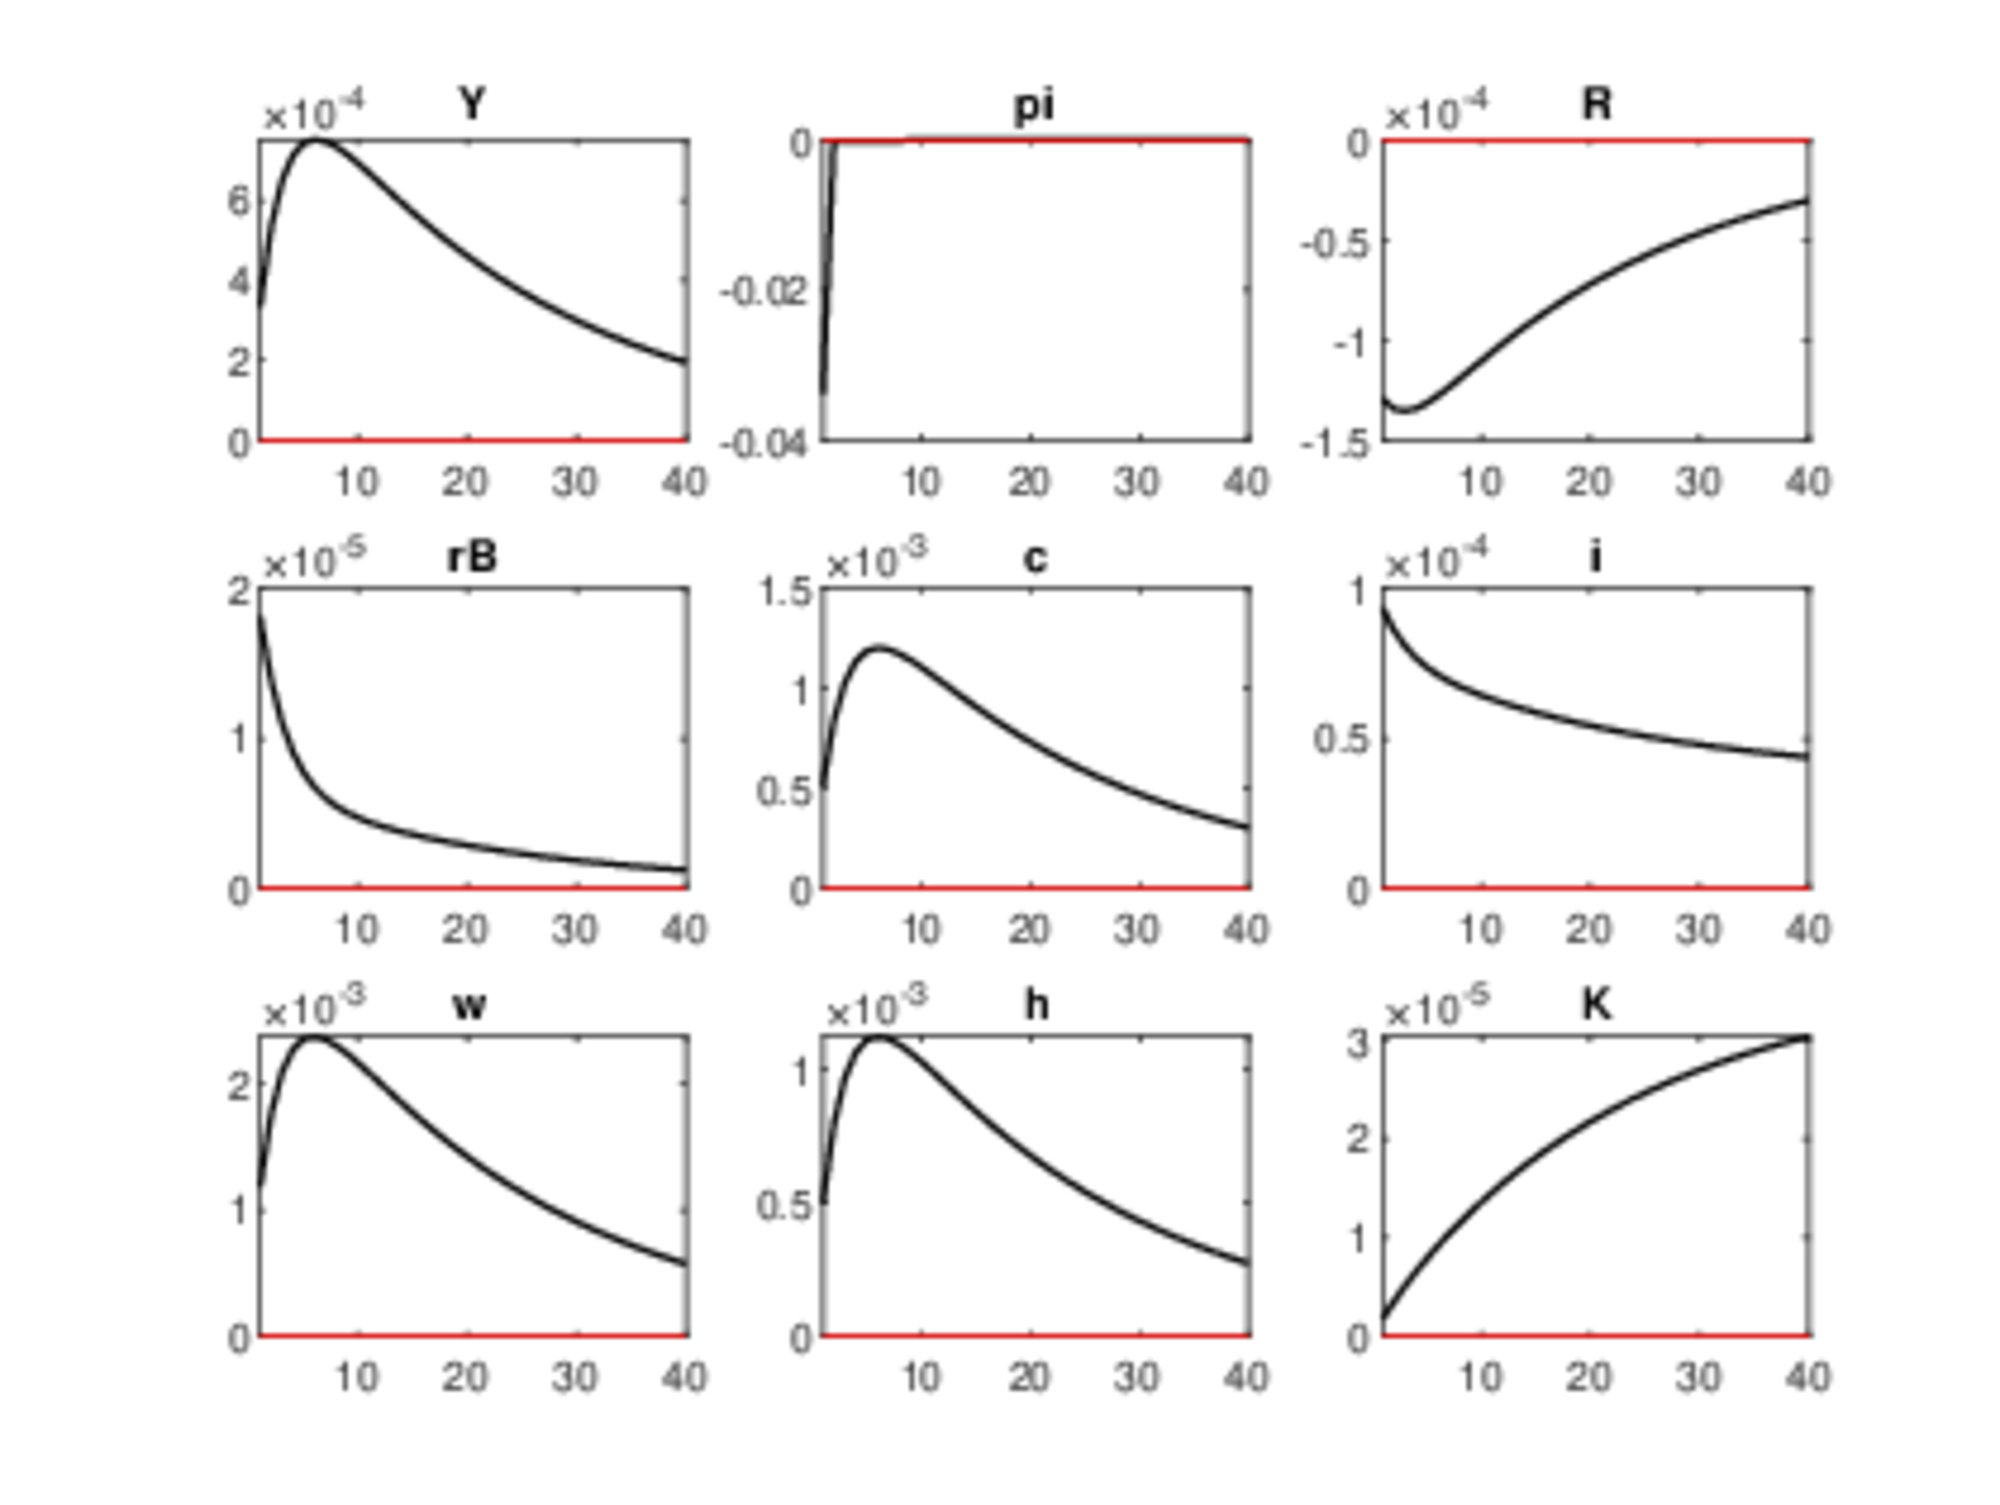
\includegraphics[width=0.7\linewidth]{data/IRF_trimmed} \caption{(mis-specified) impulse responses to a monetary policy shock in my New Keynesian model}\label{fig:unnamed-chunk-3}
\end{figure}

One likely cause is the dominance of portfolio effects, which may arise
from a large money-in-utility parameter \(\psi\) or overly restrictive
capital adjustment costs, both of which can reverse standard monetary
transmission mechanisms. Weak nominal rigidities, such as a near-zero
\(\phi_p\), flatten the Phillips Curve, severing the typical link
between inflation and marginal costs. Additionally, the high degree of
Taylor rule inertia appears to delay the policy transmission process,
reducing the immediate effectiveness of monetary interventions. These
structural frictions, together with potential parameter miscalibration,
may help explain why my impulse responses deviate so sharply from
established benchmarks.

\begin{figure}
\centering
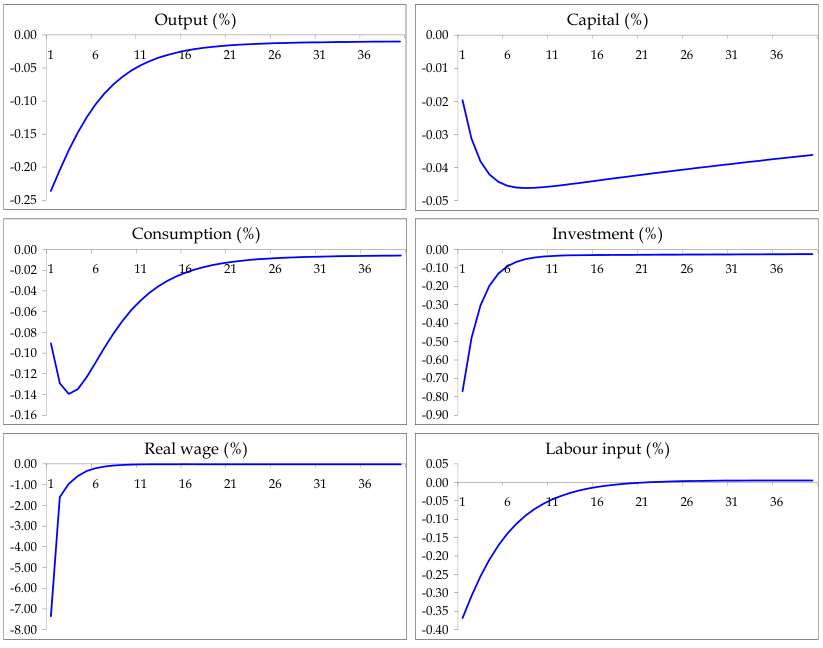
\includegraphics[width=0.6\textwidth,height=0.4\textheight]{data/dePaoli_IRF.png}
\caption{De Paoli, Scott \& Weeken (\citeproc{ref-dePaoli2007}{2007})'s
impulse responses in the sticky-price model following a monetary policy
shock}
\end{figure}

I benchmark my model against De Paoli \emph{et al.}
(\citeproc{ref-dePaoli2007}{2007}), which provides a well-structured New
Keynesian framework with sticky prices, capital adjustment costs, and
habit formation-features shared by my model. Their richer setup includes
equities, multi-period bonds, and a second-order solution to capture
risk premiums, making their results an ideal reference. In response to a
standard monetary-policy tightening, their model delivers the textbook
contraction: output, consumption, investment, real wages, hours, and
inflation all fall before gradually recovering.

By contrast, my IRFs show the opposite: my ``tightening'' raises output,
consumption, investment, hours, and capital, while inflation remains
flat and the nominal rate falls. The only structural similarity lies in
the hump-shaped capital adjustment-but with reversed sign. These
inconsistencies suggest my model either misidentifies the shock or
mis-specifies transmission mechanisms. While De Paoli's setup reinforces
the contractionary logic through richer asset pricing, mine fails to
deliver the intended dynamics - highlighting my poor MATLAB and Dynare
skills.

\newpage

\section{Appendix}\label{appendix}

\begingroup
\footnotesize

\subsection{Households}\label{households-1}

\begin{align*}
  & \text{Define Lagrangian} \\
  & \mathcal{L} = \mathbb{E}_0 \sum_{t=1}^{\infty} \beta^{t-1} \Bigl\{
    \underbrace{\frac{\bigl(c_t-\eta \, c_{t-1}\bigr)^{1-\theta}}{1-\theta}}_{\text{Consumption utility}}
    - \underbrace{\chi\frac{h_t^{1+\gamma}}{1+\gamma}}_{\text{Labour disutility}}
    + \underbrace{\psi\ln\bigl(m_t\bigr)}_{\text{Money utility}} \\
  & \quad\qquad
    + \underbrace{\lambda_t\bigl[\dfrac{R^B_{t-1}b_{t-1}}{\pi_t} + \dfrac{m_{t-1}}{\pi_t} + w_t h_t + r^k_t K_{t-1} + \Pi^r_t - \tau_t -c_t - i_t - b_t - m_t\bigr]}_{\text{Real flow constraint}}
    + \underbrace{\mu_t\bigl[(1 - \delta)\,K_{t-1}
\;+\; i_t
\;-\;\frac{\phi_k}{2}
\left(\frac{i_t}{K_{t-1}} - \delta\right)^{2}
\,K_{t-1} - K_t]}_{\text{Capital accumulation}}
  \Bigr\}
\end{align*}

\subsubsection{\texorpdfstring{First Order Conditions
\label{household_FOC}}{First Order Conditions }}\label{first-order-conditions}

FOC w.r.t. Consumption

\begin{align*}
  & \frac{\partial \mathcal{L}}{\partial c_t} = 0 \\
  & \quad \bigl[(c_t-\eta c_{t-1})^{-\theta} - \lambda_t\bigr] 
    - \beta\,\eta\,\mathbb{E}_t\bigl[(c_{t+1}-\eta c_t)^{-\theta}\bigr] = 0 \\[6pt]
  & \text{Rearrange} \\
  & \quad \lambda_t = (c_t-\eta c_{t-1})^{-\theta} - \beta\,\eta\,\mathbb{E}_t\bigl[(c_{t+1}-\eta c_t)^{-\theta}\bigr]
\end{align*}

\begin{equation}\label{foc_C_app}
\boxed{\lambda_t = (c_t-\eta c_{t-1})^{-\theta} - \beta\,\eta\,\mathbb{E}_t\bigl[(c_{t+1}-\eta c_t)^{-\theta}\bigr]}
\end{equation}

FOC w.r.t. Labour \begin{align*}
  & \frac{\partial \mathcal{L}}{\partial h_t} = 0 \\
  & \quad -\chi h_t^{\gamma} + \lambda_t w_t = 0 \\[6pt]
  & \text{Rearrange} \\
  & \quad \lambda_t w_t = \chi h_t^{\gamma}
\end{align*}

\begin{equation}\label{foc_h_app}
\boxed{\lambda_t w_t = \chi h_t^{\gamma}}
\end{equation}

FOC w.r.t. Real Bonds: \begin{align*}
  & \frac{\partial \mathcal{L}}{\partial b_t} = 0 \\
  & \quad -\beta^{t-1} \lambda_t + \beta^{t} \, \mathbb{E}_t \left[ \lambda_{t+1} \cdot \dfrac{R^B_t}{\pi_{t+1}} \right] = 0 \\[6pt]
  & \text{Divide by } \beta^{t-1} \\
  & \quad -\lambda_t + \beta \, \mathbb{E}_t \left[ \lambda_{t+1} \dfrac{R^B_t}{\pi_{t+1}} \right] = 0
\end{align*}

\begin{equation}\label{foc_B_app}
\boxed{\lambda_t = \beta \, \mathbb{E}_t \left[ \lambda_{t+1} \dfrac{R^B_t}{\pi_{t+1}} \right]}
\end{equation}

FOC w.r.t. Real Money Balances: \begin{align*}
  & \frac{\partial \mathcal{L}}{\partial m_t} = 0 \\
  & \quad \beta^{t-1} \left[ \dfrac{\psi}{m_t} - \lambda_t \right] + \beta^{t} \, \mathbb{E}_t \left[ \lambda_{t+1} \cdot \dfrac{1}{\pi_{t+1}} \right] = 0 \\[6pt]
  & \text{Divide by } \beta^{t-1} \\
  & \quad \dfrac{\psi}{m_t} - \lambda_t + \beta \, \mathbb{E}_t \left[ \dfrac{\lambda_{t+1}}{\pi_{t+1}} \right] = 0
\end{align*}

\begin{equation}\label{foc_M_app}
\boxed{\dfrac{\psi}{m_t} = \lambda_t - \beta \, \mathbb{E}_t \left[ \dfrac{\lambda_{t+1}}{\pi_{t+1}} \right]}
\end{equation}

FOC w.r.t. Investment: \begin{align*}
  & \frac{\partial \mathcal{L}}{\partial i_t} = 0 \\
  & \quad \beta^{t-1} \left[ -\lambda_t + \mu_t \cdot \frac{\partial}{\partial i_t} \left( i_t - \frac{\phi_k}{2} \left( \frac{i_t}{K_{t-1}} - \delta \right)^2 K_{t-1} \right) \right] = 0 \\[6pt]
  & \text{Compute derivative:} \\
  & \quad \frac{\partial}{\partial i_t} \left[ i_t - \frac{\phi_k}{2} \left( \frac{i_t}{K_{t-1}} - \delta \right)^2 K_{t-1} \right] = 1 - \phi_k \left( \frac{i_t}{K_{t-1}} - \delta \right) \\[6pt]
  & \text{Substitute and simplify:} \\
  & \quad -\lambda_t + \mu_t \left( 1 - \phi_k \left( \frac{i_t}{K_{t-1}} - \delta \right) \right) = 0
\end{align*}

\begin{equation}\label{foc_I_app}
\boxed{\lambda_t = \mu_t \left( 1 - \phi_k \left( \frac{i_t}{K_{t-1}} - \delta \right) \right)}
\end{equation}

FOC w.r.t. Capital: \begin{align*}
  & \frac{\partial \mathcal{L}}{\partial K_t} = 0 \\
  & \quad \beta^{t-1} (-\mu_t) + \beta^{t} \, \mathbb{E}_t \left[ \lambda_{t+1} r^k_{t+1} + \mu_{t+1} \cdot \frac{\partial}{\partial K_t} \left( (1-\delta) K_t + i_{t+1} - \frac{\phi_k}{2} \left( \frac{i_{t+1}}{K_t} - \delta \right)^2 K_t \right) \right] = 0 \\[6pt]
  & \text{Compute derivative:} \\
  & \quad \frac{\partial}{\partial K_t} \left[ (1-\delta) K_t - \frac{\phi_k}{2} \left( \frac{i_{t+1}}{K_t} - \delta \right)^2 K_t \right] = (1-\delta) - \frac{\phi_k}{2} \left( \delta^2 - \left( \frac{i_{t+1}}{K_t} \right)^2 \right) \\[6pt]
  & \text{Substitute and simplify:} \\
  & \quad -\mu_t + \beta \, \mathbb{E}_t \left[ \lambda_{t+1} r^k_{t+1} + \mu_{t+1} \left( (1-\delta) - \frac{\phi_k}{2} \left( \delta^2 - \left( \frac{i_{t+1}}{K_t} \right)^2 \right) \right) \right] = 0
\end{align*}

\begin{equation}\label{foc_K_app}
\boxed{\mu_t = \beta \, \mathbb{E}_t \left[ \lambda_{t+1} r^k_{t+1} + \mu_{t+1} \left( (1-\delta) - \frac{\phi_k}{2} \left( \delta^2 - \left( \frac{i_{t+1}}{K_t} \right)^2 \right) \right) \right]}
\end{equation}

\newpage

\subsection{Production}\label{production-1}

\subsubsection{\texorpdfstring{Final Good Producer
\label{final_good_producer_appendix}}{Final Good Producer }}\label{final-good-producer}

\textbf{Derivation of Intermediate Goods Demand and Aggregate Price
Index}

\begin{align*}  
& \text{Final goods producer's profit:} \\  
& \Pi_t = P_t Y_t - \int_0^1 P_t(j) Y_t(j)  dj \\  
& \text{subject to } Y_t = \left( \int_0^1 Y_t(j)^{\frac{\epsilon-1}{\epsilon}}  dj \right)^{\frac{\epsilon}{\epsilon-1}} \\  
& \\  
& \text{Substitute production function into profit:} \\  
& \Pi_t = P_t \left( \int_0^1 Y_t(j)^{\frac{\epsilon-1}{\epsilon}}  dj \right)^{\frac{\epsilon}{\epsilon-1}} - \int_0^1 P_t(j) Y_t(j)  dj \\  
& \\  
& \text{First-order condition for } Y_t(j): \\  
& \frac{\partial \Pi_t}{\partial Y_t(j)} = P_t \cdot \frac{\epsilon}{\epsilon-1} \left( \int_0^1 Y_t(i)^{\frac{\epsilon-1}{\epsilon}}  di \right)^{\frac{1}{\epsilon-1}} \cdot \frac{\epsilon-1}{\epsilon} Y_t(j)^{-\frac{1}{\epsilon}} - P_t(j) = 0 \\  
& \Rightarrow P_t \cdot Y_t^{\frac{1}{\epsilon}} Y_t(j)^{-\frac{1}{\epsilon}} = P_t(j) \\  
& \\  
& \text{Rearrange to obtain demand curve:} \\  
& Y_t(j) = \left( \frac{P_t}{P_t(j)} \right)^{\epsilon} Y_t \\  
& \\  
& \text{Substitute demand into production function:} \\  
& Y_t = \left( \int_0^1 \left[ \left( \frac{P_t}{P_t(j)} \right)^{\epsilon} Y_t \right]^{\frac{\epsilon-1}{\epsilon}}  dj \right)^{\frac{\epsilon}{\epsilon-1}} \\  
& = Y_t \left( \int_0^1 \left( \frac{P_t}{P_t(j)} \right)^{\epsilon-1}  dj \right)^{\frac{\epsilon}{\epsilon-1}} \\  
& \\
\end{align*}

\begin{align*} 
& \text{Simplify to obtain price index:} \\  
& 1 = \left( \int_0^1 \left( \frac{P_t}{P_t(j)} \right)^{\epsilon-1}  dj \right)^{\frac{\epsilon}{\epsilon-1}} \\  
& \Rightarrow P_t^{1-\epsilon} = \int_0^1 P_t(j)^{1-\epsilon}  dj \\  
& \Rightarrow P_t = \left( \int_0^1 P_t(j)^{1-\epsilon}  dj \right)^{\frac{1}{1-\epsilon}}  
\end{align*}

\begin{equation}\label{demand_and_price}  
\boxed{  
  \begin{gathered}  
  Y_t(j) = \left( \frac{P_t(j)}{P_t} \right)^{-\epsilon} Y_t \\  
  \\  
  P_t = \left( \int_0^1 P_t(j)^{1-\epsilon}  dj \right)^{\frac{1}{1-\epsilon}}  
  \end{gathered}  
}  
\end{equation}

\subsubsection{\texorpdfstring{Intermediate Goods Producers
\label{intermediate_good_producer_appendix}}{Intermediate Goods Producers }}\label{intermediate-goods-producers-1}

\begin{align*}
& \text{Cost minimization for intermediate firm } j: \\
& \min_{K_t(j), h_t(j)} \left\{ r_t^k K_t(j) + w_t h_t(j) \right\} \\
& \text{subject to } Y_t(j) = A_t K_t(j)^{\alpha} h_t(j)^{1-\alpha} \\
& \\
& \text{Lagrangian:} \\
& \mathcal{L} = r_t^k K_t(j) + w_t h_t(j) + \lambda_t \left[ A_t K_t(j)^{\alpha} h_t(j)^{1-\alpha} - Y_t(j) \right] \\
& \\
& \text{First-order conditions:} \\
& \frac{\partial \mathcal{L}}{\partial K_t(j)} = 0: \quad r_t^k = \lambda_t \alpha A_t K_t(j)^{\alpha-1} h_t(j)^{1-\alpha} \\
& \frac{\partial \mathcal{L}}{\partial h_t(j)} = 0: \quad w_t = \lambda_t (1-\alpha) A_t K_t(j)^{\alpha} h_t(j)^{-\alpha} \\
& \\
& \text{Rearrange FOCs:} \\
& \lambda_t = \frac{r_t^k}{\alpha} \left( \frac{K_t(j)}{h_t(j)} \right)^{1-\alpha} \frac{1}{A_t}, \quad 
\lambda_t = \frac{w_t}{1-\alpha} \left( \frac{K_t(j)}{h_t(j)} \right)^{\alpha} \frac{1}{A_t} \\
& \\
& \text{Equate expressions:} \\
& \frac{r_t^k}{\alpha} \left( \frac{K_t(j)}{h_t(j)} \right)^{-\alpha} = \frac{w_t}{1-\alpha} \left( \frac{K_t(j)}{h_t(j)} \right)^{1-\alpha} \\
& \Rightarrow \frac{K_t(j)}{h_t(j)} = \frac{\alpha}{1-\alpha} \frac{w_t}{r_t^k} \\
& \\
& \text{Substitute into capital FOC:} \\
& \lambda_t = \frac{r_t^k}{\alpha A_t} \left( \frac{\alpha}{1-\alpha} \frac{w_t}{r_t^k} \right)^{\alpha-1} \\
& = \frac{1}{A_t} \left( \frac{r_t^k}{\alpha} \right)^{\alpha} \left( \frac{w_t}{1-\alpha} \right)^{1-\alpha}
\end{align*}

\begin{equation}\label{marginal_cost_appendix}
\boxed{mc_t = \dfrac{1}{A_t} \left( \dfrac{r_t^k}{\alpha} \right)^{\alpha} \left( \dfrac{w_t}{1-\alpha} \right)^{1-\alpha}}
\end{equation}

\begin{align*}
& \text{Intermediate‐goods producer’s problem:} \\
& \max_{P_t(j)} \;\mathbb{E}_t \sum_{s=0}^{\infty} \Lambda_{t,t+s}
  \Bigl[
    \bigl(\tfrac{P_{t+s}(j)}{P_{t+s}}\bigr)^{1-\epsilon} Y_{t+s}
    - mc_{t+s}\,\bigl(\tfrac{P_{t+s}(j)}{P_{t+s}}\bigr)^{-\epsilon} Y_{t+s}
    - \tfrac{\phi_p}{2}\bigl(\tfrac{P_{t+s}(j)}{P_{t+s-1}(j)} - 1\bigr)^2 Y_{t+s}
  \Bigr] \\
& \text{subject to} \quad Y_t(j) = \bigl(\tfrac{P_t(j)}{P_t}\bigr)^{-\epsilon} Y_t
\\[1.5ex]
& \text{First‐Order Condition w.r.t. }P_t(j): \\
& \mathbb{E}_t\Bigl[
    \frac{\partial \Pi_t(j)}{\partial P_t(j)}
    + \beta\,\Lambda_{t,t+1}
      \frac{\partial \Pi_{t+1}(j)}{\partial P_t(j)}
  \Bigr] = 0
\\[1ex]
& \frac{\partial \Pi_t}{\partial P_t(j)}
  = (1-\epsilon)\bigl(\tfrac{P_t(j)}{P_t}\bigr)^{-\epsilon}\tfrac{Y_t}{P_t}
    + \epsilon\,mc_t\bigl(\tfrac{P_t(j)}{P_t}\bigr)^{-\epsilon-1}\tfrac{Y_t}{P_t}
    - \phi_p\bigl(\tfrac{P_t(j)}{P_{t-1}(j)}-1\bigr)\tfrac{Y_t}{P_{t-1}(j)}
\\[1ex]
& \frac{\partial \Pi_{t+1}}{\partial P_t(j)}
  = \phi_p\bigl(\tfrac{P_{t+1}(j)}{P_t(j)}-1\bigr)\,\tfrac{P_{t+1}(j)}{P_t(j)^2}\,Y_{t+1}
\\[2ex]
& \text{Impose symmetry: }P_t(j)=P_t,\;Y_t(j)=Y_t,\;\pi_t=\tfrac{P_t}{P_{t-1}}.\\
& (1-\epsilon)+\epsilon\,mc_t = \epsilon\bigl(mc_t-\tfrac{\epsilon-1}{\epsilon}\bigr),\quad
  \tfrac{P_t(j)}{P_{t-1}(j)}=\pi_t,\;\tfrac{P_{t+1}(j)}{P_t(j)}=\pi_{t+1}
\\[1ex]
& 0 = \epsilon\bigl(mc_t-\tfrac{\epsilon-1}{\epsilon}\bigr)
      - \phi_p\,(\pi_t-1)\,\pi_t
      + \beta\,\mathbb{E}_t\Bigl[
          \Lambda_{t,t+1}\,\phi_p\,(\pi_{t+1}-1)\,\pi_{t+1}
          \,\tfrac{Y_{t+1}P_t}{Y_tP_{t+1}}
        \Bigr]
\\[1ex]
\end{align*}

Noting \(\Lambda_{t,t+1}=\beta\,\tfrac{\lambda_{t+1}}{\lambda_t}\) and
\(P_{t+1}/P_t=\pi_{t+1}\), the bracket simplifies to
\(\beta\,\tfrac{\lambda_{t+1}}{\lambda_t}\,\tfrac{Y_{t+1}}{Y_t}\).

\begin{equation}\label{rotemberg_FOC}
\boxed{
  0 = \epsilon\Bigl(mc_t - \tfrac{\epsilon-1}{\epsilon}\Bigr)
      - \phi_p\,(\pi_t - 1)\,\pi_t
      + \beta\,\mathbb{E}_t\!
        \Bigl[
          \tfrac{\lambda_{t+1}}{\lambda_t}\,
          \phi_p\,(\pi_{t+1}-1)\,\pi_{t+1}\,
          \tfrac{Y_{t+1}}{Y_t}
        \Bigr]
}
\end{equation}

\newpage

\subsection{\texorpdfstring{Steady State
\label{steady_state_app}}{Steady State }}\label{steady-state-1}

\begin{align*}
\max_{P_t(j)}\;&(P_t(j)/P_t)^{1-\epsilon}Y_t \;-\; mc_t\,(P_t(j)/P_t)^{-\epsilon}Y_t \\[6pt]
\frac{\partial}{\partial P_t(j)}:\;&(1-\epsilon)(P_t(j)/P_t)^{-\epsilon}\frac{Y_t}{P_t}
\;+\;\epsilon\,mc_t\,(P_t(j)/P_t)^{-\epsilon-1}\frac{Y_t}{P_t}=0 \\[6pt]
\Rightarrow\;&(1-\epsilon)+\epsilon\,mc_t\,(P_t(j)/P_t)^{-1}=0 \\[4pt]
\Rightarrow\;&P_t(j)/P_t=\frac{\epsilon}{\epsilon-1}\;mc_t
\end{align*}

In equilibrium \(P_t(j)=P_t\), so \[
1=\frac{\epsilon}{\epsilon-1}\,mc_t
\] \begin{equation}\label{eq:mc}
mc^*=\frac{\epsilon-1}{\epsilon}
\end{equation}

\begin{align*}
& \text{Factor Prices and Technology Link} \\
& mc^* = \frac{\epsilon - 1}{\epsilon} \\
& r^{k,*} = \frac{1}{\beta} - (1 - \delta) \\
& mc^* = \frac{1}{A} \left( \frac{r^{k,*}}{\alpha} \right)^{\alpha}
            \left( \frac{w^*}{1-\alpha} \right)^{1-\alpha} \\
& \text{Substitute to get} \\
& \frac{\epsilon - 1}{\epsilon}
  = \frac{1}{A} \left( \frac{r^{k,*}}{\alpha} \right)^{\alpha}
    \left( \frac{w^*}{1-\alpha} \right)^{1-\alpha}
\end{align*}

\begin{align*}
& \text{Solve for Capital-Labor Ratio} \\
& k = \left(\frac{mc^*\alpha A}{r^{k,*}}\right)^{\!\frac{1}{1-\alpha}}
\end{align*}

\begin{align*}
& \text{Solve for Real Wage} \\
& w^* = mc^*(1-\alpha)Ak^\alpha
\end{align*}

\begin{align*}
& \text{Labour Supply with Habit Formation} \\
& \lambda^* = [c^*(1-\eta)]^{-\theta}(1 - \beta\eta) \\
& [c^*(1-\eta)]^{-\theta}(1 - \beta\eta)w^* = \chi(h^*)^\gamma \\[6pt]
& \Rightarrow (Ak^\alpha - \delta k)h^* - \bar{g}
= \frac{1}{1-\eta}\left(\frac{(1-\beta\eta)w^*}{\chi}\right)^{\!1/\theta}(h^*)^{-\gamma/\theta}
\end{align*}

\begin{align*}
& \text{Resource Constraints} \\
& K^* = kh^* \\
& Y^* = Ak^\alpha h^* \\
& c^* = Y^* - \delta K^* - \bar{g} \\
& i^* = \delta K^*
\end{align*}

\begin{align*}
& \text{Monetary Policy Steady State} \\
& R^* = \frac{\pi_*}{\beta}
\end{align*}

\begin{equation}\label{closed_form_ss}
\boxed{
  \begin{gathered}
    k = \left(\frac{mc^*\alpha A}{r^{k,*}}\right)^{\!1/(1-\alpha)}, 
    \quad
    r^{k,*} = 1/\beta - (1-\delta),
    \\[4pt]
    w^* = mc^*(1-\alpha)Ak^\alpha,
    \\[4pt]
    h^*:\; (Ak^\alpha - \delta k)h^* - \bar{g}
    = \frac{1}{1-\eta}\left(\frac{(1-\beta\eta)w^*}{\chi}\right)^{\!1/\theta}(h^*)^{-\gamma/\theta},
    \\[4pt]
    K^* = kh^*, 
    \quad 
    Y^* = Ak^\alpha h^*, 
    \\[4pt]
    c^* = Y^* - \delta K^* - \bar{g}, 
    \quad 
    i^* = \delta K^*,
    \\[4pt]
    R^* = \pi_*/\beta
  \end{gathered}
}
\end{equation}

\newpage

\subsection{Log-Linearisation}\label{log-linearisation}

Linearisation of Flow Constraint (Real) - Eq \ref{flow_constraint_real}
\begin{align*}
& \text{Define real wealth: } \Omega_t \equiv r^B_{t-1}b_{t-1} + \frac{m_{t-1}}{\pi_t} + w_t h_t + r^k_t K_{t-1} + \Pi^r_t - \tau_t \\[6pt]
& \text{Take total differential around steady state} \\
& \quad d(c_t) + d(i_t) + d(b_t) + d(m_t) = d\Omega_t \\[6pt]
& \text{Expand differentials using product rules} \\
& \quad dc_t + di_t + db_t + dm_t = b_{t-1}dr^B_{t-1} + r^B_{t-1}db_{t-1} + \frac{1}{\pi_t}dm_{t-1} + m_{t-1}d\left(\pi_t^{-1}\right) \\
& \qquad + h_t dw_t + w_t dh_t + K_{t-1}dr^k_t + r^k_t dK_{t-1} + d\Pi^r_t - d\tau_t \\[6pt]
& \text{Apply } d(\pi_t^{-1}) = -\pi_t^{-2}d\pi_t \text{ and steady state } \bar{\pi}=1 \\
& \quad dc_t + di_t + db_t + dm_t = \bar{b}dr^B_{t-1} + \bar{r}^B db_{t-1} + \bar{m}dm_{t-1} - \bar{m}d\pi_t \\
& \qquad + \bar{h}dw_t + \bar{w}dh_t + \bar{K}dr^k_t + \bar{r}^k dK_{t-1} + d\Pi^r_t - d\tau_t \\[6pt]
& \text{Convert to log-deviations } (\hat{x}_t \approx \frac{x_t - \bar{x}}{\bar{x}}) \\
& \quad \bar{C}\hat{c}_t + \bar{I}\hat{i}_t + \bar{B}\hat{b}_t + \bar{M}\hat{m}_t = \bar{r}^B\bar{B}\hat{r}^B_{t-1} + \bar{r}^B\bar{B}\hat{b}_{t-1} + \bar{M}\hat{m}_{t-1} - \bar{M}\hat{\pi}_t \\
& \qquad + \bar{w}\bar{H}\hat{w}_t + \bar{w}\bar{H}\hat{h}_t + \bar{r}^k\bar{K}\hat{r}^k_t + \bar{r}^k\bar{K}\hat{K}_{t-1} + \overline{\Pi}^r \widehat{\Pi}^r_t - \bar{T}\hat{\tau}_t
\end{align*}

\begin{equation}\label{flow_constraint_real_linearised_app}
\boxed{
\begin{aligned}
\bar{C}\hat{c}_t + \bar{I}\hat{i}_t &+ \bar{B}\hat{b}_t + \bar{M}\hat{m}_t = \\
&\bar{r}^B\bar{B}(\hat{r}^B_{t-1} + \hat{b}_{t-1}) + \bar{M}(\hat{m}_{t-1} - \hat{\pi}_t) \\
&+ \bar{w}\bar{H}(\hat{w}_t + \hat{h}_t) + \bar{r}^k\bar{K}(\hat{r}^k_t + \hat{K}_{t-1}) \\
&+ \overline{\Pi}^r \widehat{\Pi}^r_t - \bar{T}\hat{\tau}_t
\end{aligned}
}
\end{equation}

Linearisation of Capital Accumulation - Eq
\ref{capital_accumulation_real} \begin{align*}
& \text{Define investment ratio: } z_t \equiv i_t/K_{t-1} \\[6pt]
& \text{Rewrite equation: } K_t = (1-\delta)K_{t-1} + i_t - \frac{\phi_k}{2}(z_t - \delta)^2 K_{t-1} \\[6pt]
& \text{Steady state: } \bar{z} = \delta \implies \bar{K} = (1-\delta)\bar{K} + \bar{I} \\[6pt]
& \text{Take total differential:} \\
& \quad dK_t = (1-\delta)dK_{t-1} + di_t - \phi_k(z_t - \delta)K_{t-1}dz_t - \frac{\phi_k}{2}(z_t - \delta)^2 dK_{t-1} \\[6pt]
& \text{Evaluate at } \bar{z}=\delta: \\
& \quad dK_t = (1-\delta)dK_{t-1} + di_t \\[6pt]
& \text{Convert to log-deviations:} \\
& \quad \bar{K}\hat{K}_t = (1-\delta)\bar{K}\hat{K}_{t-1} + \bar{I}\hat{i}_t \\[6pt]
& \text{Divide by } \bar{K} \text{ and use } \delta \equiv \bar{I}/\bar{K}: \\
& \quad \hat{K}_t = (1-\delta)\hat{K}_{t-1} + \delta \hat{i}_t
\end{align*}

\begin{equation}\label{capital_accumulation_real_linearised_app}
\boxed{\hat{K}_t = (1-\delta)\hat{K}_{t-1} + \delta \hat{i}_t}
\end{equation}

Linearisation of Firm Profits - Eq \ref{intermediate_firm_profit_real}
\begin{align*}
& \text{Define price adjustment cost: } \Phi_t \equiv \frac{\phi_p}{2}(\pi_t - 1)^2 Y_t \\[6pt]
& \text{Steady state: } \bar{\pi}=1 \implies \bar{\Phi}=0 \\[6pt]
& \text{Take total differential:} \\
& \quad d\Pi^r_t = dY_t - d(r^k_t K_{t-1}) - d(w_t h_t) - d\Phi_t \\[6pt]
& \text{Expand factor payments:} \\
& \quad = dY_t - (K_{t-1}dr^k_t + r^k_t dK_{t-1}) - (h_t dw_t + w_t dh_t) - d\Phi_t \\[6pt]
& \text{Differentiate adjustment cost:} \\
& \quad d\Phi_t = \phi_p(\pi_t - 1)d\pi_t Y_t + \frac{\phi_p}{2}(\pi_t - 1)^2 dY_t \\[6pt]
& \text{Evaluate at } \bar{\pi}=1: \\
& \quad d\Phi_t = 0 \\[6pt]
& \text{Convert to log-deviations:} \\
& \quad \overline{\Pi}^r \widehat{\Pi}^r_t = \bar{Y}\hat{Y}_t - \bar{r}^k\bar{K}\hat{r}^k_t - \bar{r}^k\bar{K}\hat{K}_{t-1} - \bar{w}\bar{H}\hat{w}_t - \bar{w}\bar{H}\hat{h}_t
\end{align*}

\begin{equation}\label{intermediate_firm_profit_real_linearised_app}
\boxed{\widehat{\Pi}^r_t = \frac{\bar{Y}}{\overline{\Pi}^r}\hat{Y}_t - \frac{\bar{r}^k\bar{K}}{\overline{\Pi}^r}(\hat{r}^k_t + \hat{K}_{t-1}) - \frac{\bar{w}\bar{H}}{\overline{\Pi}^r}(\hat{w}_t + \hat{h}_t)}
\end{equation}

Linearisation of FOC Consumption - Eq \ref{foc_C} \begin{align*}
& \text{Define habit-adjusted consumption:} \\
& \quad s_t \equiv c_t - \eta c_{t-1}, \quad s_{t+1} \equiv c_{t+1} - \eta c_t \\[6pt]
& \text{Original equation: } \lambda_t = s_t^{-\theta} - \beta\eta \mathbb{E}_t [s_{t+1}^{-\theta}] \\[6pt]
& \text{Steady state: } \bar{\lambda} = (1 - \beta\eta)\bar{s}^{-\theta} \\[6pt]
& \text{Take total differential:} \\
& \quad d\lambda_t = -\theta s_t^{-\theta-1} ds_t + \beta\eta \theta \mathbb{E}_t [s_{t+1}^{-\theta-1} ds_{t+1}] \\[6pt]
& \text{Expand differentials:} \\
& \quad ds_t = dc_t - \eta dc_{t-1}, \quad ds_{t+1} = dc_{t+1} - \eta dc_t \\[6pt]
& \text{Evaluate at steady state } (s_t = s_{t+1} = \bar{s}): \\
& \quad d\lambda_t = -\theta \bar{s}^{-\theta-1} (dc_t - \eta dc_{t-1}) + \beta\eta \theta \bar{s}^{-\theta-1} \mathbb{E}_t [dc_{t+1} - \eta dc_t] \\[6pt]
& \text{Convert to log-deviations:} \\
& \quad \bar{\lambda}\hat{\lambda}_t = -\theta \bar{s}^{-\theta-1} \bar{C} (\hat{c}_t - \eta \hat{c}_{t-1}) + \beta\eta \theta \bar{s}^{-\theta-1} \bar{C} \mathbb{E}_t [\hat{c}_{t+1} - \eta \hat{c}_t] \\[6pt]
& \text{Simplify using } \bar{s} = \bar{C}(1-\eta) \text{ and } \bar{\lambda} = (1-\beta\eta)\bar{s}^{-\theta}: \\
& \quad \hat{\lambda}_t = -\frac{\theta}{(1-\eta)} \left[ (\hat{c}_t - \eta \hat{c}_{t-1}) - \beta\eta \mathbb{E}_t (\hat{c}_{t+1} - \eta \hat{c}_t) \right]
\end{align*}

\begin{equation}\label{foc_C_linearised_app}
\boxed{\hat{\lambda}_t = -\frac{\theta}{(1-\eta)} \left( \hat{c}_t - \eta \hat{c}_{t-1} - \beta\eta \mathbb{E}_t \left[\hat{c}_{t+1} - \eta \hat{c}_t\right] \right)}
\end{equation}

Log-linearisation of FOC w.r.t. Labour (h\_t) - Eq \ref{foc_h}
\begin{align*}
& \text{Original equation: } \lambda_t w_t = \chi h_t^{\gamma} \\[6pt]
& \text{Take natural logarithm of both sides} \\
& \quad \ln(\lambda_t w_t) = \ln(\chi h_t^{\gamma}) \\[6pt]
& \text{Apply logarithmic identities} \\
& \quad \ln \lambda_t + \ln w_t = \ln \chi + \gamma \ln h_t \\[6pt]
& \text{Define log-deviations from steady state } (\hat{x}_t \equiv \ln x_t - \ln \bar{x}) \\
& \quad (\ln \lambda_t - \ln \bar{\lambda}) + (\ln w_t - \ln \bar{w}) = \gamma (\ln h_t - \ln \bar{h}) \\[6pt]
& \text{Recognize steady-state relationship: } \bar{\lambda}\bar{w} = \chi \bar{h}^{\gamma} \\
& \quad \Rightarrow \ln \bar{\lambda} + \ln \bar{w} = \ln \chi + \gamma \ln \bar{h} \\[6pt]
& \text{Subtract steady-state equation} \\
& \quad \hat{\lambda}_t + \hat{w}_t = \gamma \hat{h}_t
\end{align*}

\begin{equation}\label{foc_h_linearised_app}
\boxed{\hat{\lambda}_t + \hat{w}_t = \gamma \hat{h}_t}
\end{equation}

Log-linearisation of FOC for Bonds (foc\_B) \begin{align*}
& \text{Original equation: } 1 = \beta \mathbb{E}_t \left[ \frac{\lambda_{t+1}}{\lambda_t} r^B_t \right] \\[6pt]
& \text{Steady state: } 1 = \beta \frac{\bar{\lambda}}{\bar{\lambda}} \bar{r}^B \implies \bar{r}^B = 1/\beta \\[6pt]
& \text{Take natural logarithm} \\
& \quad 0 = \ln \beta + \ln \mathbb{E}_t \left[ \frac{\lambda_{t+1}}{\lambda_t} r^B_t \right] \\[6pt]
& \text{Apply certainty equivalence (}\ln \mathbb{E}_t[X] \approx \mathbb{E}_t[\ln X]\text{)} \\
& \quad 0 = \ln \beta + \mathbb{E}_t \left[ \ln \lambda_{t+1} - \ln \lambda_t + \ln r^B_t \right] \\[6pt]
& \text{Subtract steady state } (0 = \ln \beta + \ln \bar{\lambda} - \ln \bar{\lambda} + \ln \bar{r}^B) \\
& \quad 0 = \mathbb{E}_t \left[ (\ln \lambda_{t+1} - \ln \bar{\lambda}) - (\ln \lambda_t - \ln \bar{\lambda}) + (\ln r^B_t - \ln \bar{r}^B) \right] \\[6pt]
& \text{Convert to log-deviations} \\
& \quad 0 = \mathbb{E}_t \left[ \hat{\lambda}_{t+1} - \hat{\lambda}_t + \hat{r}^B_t \right]
\end{align*}

\begin{equation}\label{foc_B_linearised_app}
\boxed{\hat{r}^B_t = \hat{\lambda}_t - \mathbb{E}_t \hat{\lambda}_{t+1}}
\end{equation}

Log-linearisation of FOC for Money (foc\_M) \begin{align*}
& \text{Original: } \lambda_t = \dfrac{\psi}{m_t} + \beta \mathbb{E}_t \left[ \dfrac{\lambda_{t+1}}{\pi_{t+1}} \right] \\[6pt]
& \text{Steady state: } \bar{\lambda} = \dfrac{\psi}{\bar{m}} + \beta \dfrac{\bar{\lambda}}{\bar{\pi}} \quad (\text{with } \bar{\pi}=1) \\[6pt]
& \text{Take total differential} \\
& \quad d\lambda_t = -\dfrac{\psi}{m_t^2} dm_t + \beta \mathbb{E}_t \left[ \frac{1}{\pi_{t+1}} d\lambda_{t+1} - \frac{\lambda_{t+1}}{\pi_{t+1}^2} d\pi_{t+1} \right] \\[6pt]
& \text{Evaluate at steady state } (\bar{\pi}=1) \\
& \quad d\lambda_t = -\dfrac{\psi}{\bar{m}^2} dm_t + \beta \mathbb{E}_t \left[ d\lambda_{t+1} - \bar{\lambda} d\pi_{t+1} \right] \\[6pt]
& \text{Convert to log-deviations} \\
& \quad \bar{\lambda} \hat{\lambda}_t = -\dfrac{\psi}{\bar{m}} \hat{m}_t + \beta \mathbb{E}_t \left[ \bar{\lambda} \hat{\lambda}_{t+1} - \bar{\lambda} \hat{\pi}_{t+1} \right] \\[6pt]
& \text{Divide by } \bar{\lambda} \text{ and define } \zeta \equiv \dfrac{\psi}{\bar{m}\bar{\lambda}} \\
& \quad \hat{\lambda}_t = -\zeta \hat{m}_t + \beta \mathbb{E}_t \left[ \hat{\lambda}_{t+1} - \hat{\pi}_{t+1} \right] \\[6pt]
& \text{From steady state: } \zeta = 1 - \beta
\end{align*}

\begin{equation}\label{foc_M_linearised_app}
\boxed{\hat{\lambda}_t = -(1 - \beta) \hat{m}_t + \beta \mathbb{E}_t \left[ \hat{\lambda}_{t+1} - \hat{\pi}_{t+1} \right]}
\end{equation}

Log-linearisation of FOC for Investment (foc\_I) \begin{align*}
& \text{Original: } \mu_t = \lambda_t \left( 1 - \phi_k \left( \frac{i_t}{K_{t-1}} - \delta \right) \right)^{-1} \\[6pt]
& \text{Steady state: } \bar{\mu} = \bar{\lambda} \quad (\text{since } i_t/K_{t-1} = \delta) \\[6pt]
& \text{Rewrite as: } \frac{\mu_t}{\lambda_t} = \left( 1 - \phi_k z_t \right)^{-1} \quad \left(z_t \equiv \frac{i_t}{K_{t-1}} - \delta\right) \\[6pt]
& \text{Take natural logarithm} \\
& \quad \ln \mu_t - \ln \lambda_t = -\ln(1 - \phi_k z_t) \\[6pt]
& \text{Linearize RHS (first-order Taylor):} \\
& \quad -\ln(1 - \phi_k z_t) \approx \phi_k z_t \quad (\text{since } \bar{z}=0) \\[6pt]
& \text{Take total differential} \\
& \quad \frac{d\mu_t}{\mu_t} - \frac{d\lambda_t}{\lambda_t} = \phi_k dz_t \\[6pt]
& \text{Convert to log-deviations} \\
& \quad \hat{\mu}_t - \hat{\lambda}_t = \phi_k d\left(\frac{i_t}{K_{t-1}}\right) \\[6pt]
& \text{Expand differential:} \\
& \quad d\left(\frac{i_t}{K_{t-1}}\right) = \frac{1}{\bar{K}} di_t - \frac{\bar{i}}{\bar{K}^2} dK_{t-1} = \delta \left( \frac{di_t}{\bar{i}} - \frac{dK_{t-1}}{\bar{K}} \right) \\[6pt]
& \quad = \delta (\hat{i}_t - \hat{K}_{t-1})
\end{align*}

\begin{equation}\label{foc_I_linearised_app}
\boxed{\hat{\mu}_t = \hat{\lambda}_t + \phi_k \delta \left( \hat{i}_t - \hat{K}_{t-1} \right)}
\end{equation}

Log-linearisation of FOC for Capital (foc\_K) \begin{align*}
& \text{Original: } 1 = \beta \mathbb{E}_t \left[ \frac{\lambda_{t+1}}{\mu_t} r^k_{t+1} + \frac{\mu_{t+1}}{\mu_t} \Gamma_{t+1} \right] \\[4pt]
& \text{where } \Gamma_{t+1} \equiv (1-\delta) - \frac{\phi_k}{2} \left( \delta^2 - \left( \frac{i_{t+1}}{K_t} \right)^2 \right) \\[6pt]
& \text{Steady state: } \frac{i_{t+1}}{K_t} = \delta \implies \bar{\Gamma} = 1 - \delta \\[6pt]
& \text{Steady state equation:} \\
& \quad 1 = \beta \left[ \frac{\bar{\lambda}}{\bar{\mu}} \bar{r}^k + \frac{\bar{\mu}}{\bar{\mu}} (1-\delta) \right] = \beta \left[ \bar{r}^k + 1 - \delta \right] \quad (\text{since } \bar{\mu}=\bar{\lambda}) \\[6pt]
& \text{Take total differential} \\
& \quad 0 = \beta \mathbb{E}_t \left[ d\left( \frac{\lambda_{t+1} r^k_{t+1}}{\mu_t} \right) + d\left( \frac{\mu_{t+1} \Gamma_{t+1}}{\mu_t} \right) \right] \\[6pt]
& \text{First term: } d\left( \frac{\lambda_{t+1} r^k_{t+1}}{\mu_t} \right) = \frac{1}{\mu_t} d(\lambda_{t+1} r^k_{t+1}) - \frac{\lambda_{t+1} r^k_{t+1}}{\mu_t^2} d\mu_t \\[6pt]
& \text{Second term: } d\left( \frac{\mu_{t+1} \Gamma_{t+1}}{\mu_t} \right) = \frac{1}{\mu_t} d(\mu_{t+1} \Gamma_{t+1}) - \frac{\mu_{t+1} \Gamma_{t+1}}{\mu_t^2} d\mu_t \\[6pt]
& \text{Evaluate at steady state } (\bar{\Gamma}=1-\delta) \\[6pt]
& \quad 0 = \beta \mathbb{E}_t \left[ \frac{1}{\bar{\mu}} (\bar{r}^k d\lambda_{t+1} + \bar{\lambda} dr^k_{t+1}) - \frac{\bar{\lambda} \bar{r}^k}{\bar{\mu}^2} d\mu_t \right. \\
& \quad \left. + \frac{1}{\bar{\mu}} \left( (1-\delta) d\mu_{t+1} + \bar{\mu} d\Gamma_{t+1} \right) - \frac{\bar{\mu} (1-\delta)}{\bar{\mu}^2} d\mu_t \right] \\[6pt]
& \text{Simplify using } \bar{\mu}=\bar{\lambda}: \\
& \quad 0 = \beta \mathbb{E}_t \left[ \frac{\bar{r}^k}{\bar{\lambda}} d\lambda_{t+1} + dr^k_{t+1} - \frac{\bar{r}^k}{\bar{\lambda}} d\mu_t + \frac{1-\delta}{\bar{\lambda}} d\mu_{t+1} + d\Gamma_{t+1} - \frac{1-\delta}{\bar{\lambda}} d\mu_t \right] \\[6pt]
& \text{Differentiate } \Gamma_{t+1}: \\
& \quad d\Gamma_{t+1} = \phi_k \frac{i_{t+1}}{K_t} d\left( \frac{i_{t+1}}{K_t} \right) = \phi_k \delta \cdot d\left( \frac{i_{t+1}}{K_t} \right) \\[6pt]
& \quad d\left( \frac{i_{t+1}}{K_t} \right) = \frac{1}{\bar{K}} di_{t+1} - \frac{\bar{i}}{\bar{K}^2} dK_t = \delta (\hat{i}_{t+1} - \hat{K}_t) \\[6pt]
& \text{Convert to log-deviations:} \\
& \quad 0 = \beta \mathbb{E}_t \left[ \bar{r}^k \hat{\lambda}_{t+1} + \bar{r}^k \hat{r}^k_{t+1} - \bar{r}^k \hat{\mu}_t + (1-\delta) \hat{\mu}_{t+1} - (1-\delta) \hat{\mu}_t + \phi_k \delta^2 (\hat{i}_{t+1} - \hat{K}_t) \right] \\[6pt]
& \text{Divide by } \beta \text{ and use steady-state relation } 1 = \beta(\bar{r}^k + 1 - \delta)
\end{align*}

\begin{equation}\label{foc_K_linearised_app}
\boxed{\mathbb{E}_t \left[ \bar{r}^k (\hat{\lambda}_{t+1} + \hat{r}^k_{t+1}) + (1-\delta) \hat{\mu}_{t+1} + \phi_k \delta^2 (\hat{i}_{t+1} - \hat{K}_t) = (\bar{r}^k + 1 - \delta) \hat{\mu}_t \right]}
\end{equation}

Log-linearisation of Aggregate Production Function \begin{align*}
& \text{Original: } Y_t = A_t K_{t-1}^{\alpha} h_t^{1-\alpha} \\[6pt]
& \text{Take natural logarithm} \\
& \quad \ln Y_t = \ln A_t + \alpha \ln K_{t-1} + (1-\alpha) \ln h_t \\[6pt]
& \text{Define log-deviations } \hat{x}_t \equiv \ln x_t - \ln \bar{x} \\
& \quad (\ln Y_t - \ln \bar{Y}) = (\ln A_t - \ln \bar{A}) + \alpha (\ln K_{t-1} - \ln \bar{K}) + (1-\alpha) (\ln h_t - \ln \bar{h}) \\[6pt]
& \text{Recognize steady state: } \bar{Y} = \bar{A} \bar{K}^{\alpha} \bar{h}^{1-\alpha} \\[6pt]
& \text{Substitute deviation variables}
\end{align*}

\begin{equation}\label{aggregate_production_linearised_app}
\boxed{\hat{Y}_t = \hat{A}_t + \alpha \hat{K}_{t-1} + (1-\alpha) \hat{h}_t}
\end{equation}

Log-linearisation of Marginal Cost \begin{align*}
& \text{Original: } mc_t = \frac{1}{A_t} \left( \frac{r_t^k}{\alpha} \right)^{\alpha} \left( \frac{w_t}{1-\alpha} \right)^{1-\alpha} \\[6pt]
& \text{Take natural logarithm} \\
& \quad \ln mc_t = -\ln A_t + \alpha \ln r_t^k - \alpha \ln \alpha + (1-\alpha) \ln w_t - (1-\alpha) \ln (1-\alpha) \\[6pt]
& \text{Define log-deviations} \\
& \quad (\ln mc_t - \ln \overline{mc}) = -(\ln A_t - \ln \bar{A}) + \alpha (\ln r_t^k - \ln \bar{r}^k) + (1-\alpha) (\ln w_t - \ln \bar{w}) \\[6pt]
& \text{Recognize steady state: } \overline{mc} = \frac{1}{\bar{A}} \left( \frac{\bar{r}^k}{\alpha} \right)^{\alpha} \left( \frac{\bar{w}}{1-\alpha} \right)^{1-\alpha} \\[6pt]
& \text{Substitute deviation variables}
\end{align*}

\begin{equation}\label{marginal_cost_linearised_app}
\boxed{\widehat{mc}_t = -\hat{A}_t + \alpha \hat{r}^k_t + (1-\alpha) \hat{w}_t}
\end{equation}

Log-linearisation of NK Phillips Curve \begin{align*}
& \text{Original: } (\pi_t - 1)\pi_t = \frac{\epsilon}{\phi_p} \left( mc_t - \frac{\epsilon-1}{\epsilon} \right) + \beta \mathbb{E}_t \left[ \frac{\lambda_{t+1}}{\lambda_t} \frac{Y_{t+1}}{Y_t} (\pi_{t+1} - 1)\pi_{t+1} \right] \\[6pt]
& \text{Define auxiliary variable: } \Theta_t \equiv (\pi_t - 1)\pi_t \\[6pt]
& \text{Steady state: } \bar{\pi} = 1 \implies \bar{\Theta} = 0, \quad \overline{mc} = \frac{\epsilon-1}{\epsilon} \\[6pt]
& \text{First-order Taylor expansion around steady state:} \\[6pt]
& \text{LHS: } \Theta_t \approx 0 + \left.\frac{\partial \Theta_t}{\partial \pi_t}\right|_{\bar{\pi}} (\pi_t - 1) \\
& \quad \frac{\partial \Theta_t}{\partial \pi_t} = 2\pi_t - 1 \implies \left.\frac{\partial \Theta_t}{\partial \pi_t}\right|_{\bar{\pi}=1} = 1 \\
& \quad \Theta_t \approx \hat{\pi}_t \\[6pt]
& \text{First term RHS: } \frac{\epsilon}{\phi_p} \left( mc_t - \frac{\epsilon-1}{\epsilon} \right) \approx \frac{\epsilon}{\phi_p} \overline{mc} \widehat{mc}_t = \frac{\epsilon}{\phi_p} \cdot \frac{\epsilon-1}{\epsilon} \widehat{mc}_t = \frac{\epsilon-1}{\phi_p} \widehat{mc}_t \\[6pt]
& \text{Second term RHS: } \beta \mathbb{E}_t \left[ \frac{\lambda_{t+1}}{\lambda_t} \frac{Y_{t+1}}{Y_t} \Theta_{t+1} \right] \\[6pt]
& \quad \text{Steady state value: } \beta \mathbb{E}_t \left[ 1 \cdot 1 \cdot 0 \right] = 0 \\[6pt]
& \quad \text{Differential: } \beta \mathbb{E}_t \left[ d\left( \frac{\lambda_{t+1}}{\lambda_t} \right) \cdot 1 \cdot 0 + 1 \cdot d\left( \frac{Y_{t+1}}{Y_t} \right) \cdot 0 + 1 \cdot 1 \cdot d\Theta_{t+1} \right] \\
& \quad = \beta \mathbb{E}_t \left[ d\Theta_{t+1} \right] \approx \beta \mathbb{E}_t \hat{\pi}_{t+1} \\[6pt]
& \text{Combine results}
\end{align*}

\begin{equation}\label{nkpc_linearised_app}
\boxed{\hat{\pi}_t = \frac{\epsilon-1}{\phi_p} \widehat{mc}_t + \beta \mathbb{E}_t \hat{\pi}_{t+1}}
\end{equation}

Log-linearisation of Government Budget Constraint \begin{align*}
& \text{Assume equality in steady state: } \bar{g} + \bar{r}^B \bar{d} = \bar{d} + \bar{\tau} + \frac{\bar{m} - \bar{m}}{\bar{\pi}} \\[6pt]
& \text{Take total differential:} \\
& \quad dg_t + d(r^B_{t-1} d_{t-1}) = dd_t + d\tau_t + d\left( \frac{m_{t-1} - m_t}{\pi_t} \right) \\[6pt]
& \text{Expand compound terms:} \\
& \quad dg_t + d_{t-1} dr^B_{t-1} + r^B_{t-1} dd_{t-1} = dd_t + d\tau_t + \frac{1}{\pi_t} d(m_{t-1} - m_t) + (m_{t-1} - m_t) d\left(\frac{1}{\pi_t}\right) \\[6pt]
& \text{Apply derivative rules:} \\
& \quad d(1/\pi_t) = -\pi_t^{-2} d\pi_t \\[6pt]
& \text{Evaluate at steady state } (\bar{\pi} = 1, \bar{m}_{t-1} = \bar{m}_t = \bar{M}): \\
& \quad dg_t + \bar{d} dr^B_{t-1} + \bar{r}^B dd_{t-1} = dd_t + d\tau_t + \frac{1}{1} (dm_{t-1} - dm_t) + (0) \cdot (-\pi_t^{-2} d\pi_t) \\[6pt]
& \text{Convert to log-deviations } (\hat{x}_t \equiv \frac{x_t - \bar{x}}{\bar{x}}): \\
& \quad \bar{G} \hat{g}_t + \bar{d} \cdot \bar{r}^B \hat{r}^B_{t-1} + \bar{r}^B \bar{d} \hat{d}_{t-1} = \bar{D} \hat{d}_t + \bar{T} \hat{\tau}_t + \bar{M} \hat{m}_{t-1} - \bar{M} \hat{m}_t
\end{align*}

Log-linearisation of Resource Constraint \begin{align*}
& \text{Original: } Y_t = c_t + i_t + g_t + \frac{\phi_k}{2} \left( \frac{i_t}{K_{t-1}} - \delta \right)^2 K_{t-1} + \frac{\phi_p}{2} (\pi_t - 1)^2 Y_t \\[6pt]
& \text{Steady state: } \frac{\bar{i}}{\bar{K}} = \delta, \bar{\pi} = 1 \implies \text{ adjustment costs = 0} \\[6pt]
& \text{Take total differential:} \\
& \quad dY_t = dc_t + di_t + dg_t + d\left[ \frac{\phi_k}{2} \left( \frac{i_t}{K_{t-1}} - \delta \right)^2 K_{t-1} \right] + d\left[ \frac{\phi_p}{2} (\pi_t - 1)^2 Y_t \right] \\[6pt]
& \text{Evaluate at steady state:} \\
& \quad \text{(Adjustment cost terms vanish)} \\
& \quad dY_t = dc_t + di_t + dg_t \\[6pt]
& \text{Convert to log-deviations:} \\
& \quad \bar{Y} \hat{Y}_t = \bar{C} \hat{c}_t + \bar{I} \hat{i}_t + \bar{G} \hat{g}_t
\end{align*}

\begin{equation}\label{clearing_resource_constraint_linearised_app}
\boxed{\hat{Y}_t = \frac{\bar{C}}{\bar{Y}} \hat{c}_t + \frac{\bar{I}}{\bar{Y}} \hat{i}_t + \frac{\bar{G}}{\bar{Y}} \hat{g}_t}
\end{equation}

Log-linearisation of Bond Market Clearing \begin{align*}
& \text{Original: } b_t = d_t \\[6pt]
& \text{Take total differential:} \\
& \quad db_t = dd_t \\[6pt]
& \text{Convert to log-deviations:} \\
& \quad \bar{B} \hat{b}_t = \bar{D} \hat{d}_t \\[6pt]
& \text{Since } \bar{B} = \bar{D} \text{ in steady state:} \\
& \quad \hat{b}_t = \hat{d}_t
\end{align*}

\begin{equation}\label{Bond_market_clear_linearised_app}
\boxed{\hat{b}_t = \hat{d}_t}
\end{equation}

Log-linearisation of Fisher Equation \begin{align*}
& \text{Original: } R_t = r^B_t \cdot \mathbb{E}_t[\pi_{t+1}] \\[6pt]
& \text{Take natural logarithm:} \\
& \quad \ln R_t = \ln r^B_t + \ln \mathbb{E}_t[\pi_{t+1}] \\[6pt]
& \text{Apply certainty equivalence: } \ln \mathbb{E}_t[\pi_{t+1}] \approx \mathbb{E}_t[\ln \pi_{t+1}] \\[6pt]
& \quad \ln R_t = \ln r^B_t + \mathbb{E}_t[\ln \pi_{t+1}] \\[6pt]
& \text{Subtract steady state } (\ln \bar{R} = \ln \bar{r}^B + \ln 1): \\
& \quad (\ln R_t - \ln \bar{R}) = (\ln r^B_t - \ln \bar{r}^B) + \mathbb{E}_t[(\ln \pi_{t+1} - \ln 1)] \\[6pt]
& \text{Recognize log-deviations:}
\end{align*}

\begin{equation}\label{fisher_linearised_app}
\boxed{\hat{R}_t = \hat{r}^B_t + \mathbb{E}_t \hat{\pi}_{t+1}}
\end{equation}

Log-linearisation of Taylor Rule \begin{align*}
& \text{Define output gap: } \hat{Y}^g_t \equiv \frac{Y_t - Y_*}{Y_*} \approx \hat{Y}_t \quad (\text{since } Y_* = \bar{Y} \text{ in steady state}) \\[6pt]
& \text{Steady state: } \bar{R} = R_*, \quad \bar{\pi} = \pi_* \\[6pt]
& \text{Express in deviations:} \\
& \quad R_t - \bar{R} = \rho_R (R_{t-1} - \bar{R}) + (1 - \rho_R) \left[ \kappa_\pi (\pi_t - \bar{\pi}) + \kappa_y \hat{Y}_t \right] + \varepsilon_t^R \\[6pt]
& \text{Convert to log-deviations } (\hat{R}_t \equiv \ln R_t - \ln \bar{R} \approx \frac{R_t - \bar{R}}{\bar{R}}): \\
& \quad \bar{R} \hat{R}_t = \rho_R \bar{R} \hat{R}_{t-1} + (1 - \rho_R) \left[ \kappa_\pi \bar{\pi} \hat{\pi}_t + \kappa_y \bar{Y} \hat{Y}_t \right] + \varepsilon_t^R \\[6pt]
& \text{Divide by } \bar{R} \text{ and use } \bar{\pi} = 1:
\end{align*}

\begin{equation}\label{taylor_rule_linearised_app}
\boxed{\hat{R}_t = \rho_R \hat{R}_{t-1} + \frac{(1 - \rho_R)}{\bar{R}} \left( \kappa_\pi \hat{\pi}_t + \kappa_y \bar{Y} \hat{Y}_t \right) + \frac{\varepsilon_t^R}{\bar{R}}}
\end{equation}

Log-linearisation of Tax Rule \begin{align*}
& \text{Define deviation: } \hat{\tau}_t \equiv \frac{\tau_t - \bar{\tau}}{\bar{T}} \\[6pt]
& \text{Original: } \tau_t - \bar{\tau} = \rho_\tau (\tau_{t-1} - \bar{\tau}) + \varepsilon_t^\tau \\[6pt]
& \text{Divide by steady-state taxes } \bar{T} = \bar{\tau}: \\
& \quad \frac{\tau_t - \bar{\tau}}{\bar{T}} = \rho_\tau \frac{\tau_{t-1} - \bar{\tau}}{\bar{T}} + \frac{\varepsilon_t^\tau}{\bar{T}}
\end{align*}

\begin{equation}\label{real_taxes_linearised_app}
\boxed{\hat{\tau}_t = \rho_\tau \hat{\tau}_{t-1} + \varepsilon_t^\tau}
\text{where } \varepsilon_t^\tau \text{ is redefined as } \frac{\text{original shock}}{\bar{T}}
\end{equation}

Log-linearisation of Government Spending Process \begin{align*}
& \text{Original: } g_t = (1-\rho_g)\bar{g} + \rho_g g_{t-1} + \varepsilon_t^g \\[6pt]
& \text{Define log-deviation: } \hat{g}_t \equiv \frac{g_t - \bar{g}}{\bar{G}} \\[6pt]
& \text{Subtract steady state:} \\
& \quad g_t - \bar{g} = \rho_g (g_{t-1} - \bar{g}) + \varepsilon_t^g \\[6pt]
& \text{Divide by } \bar{G} \text{ (where } \bar{G} = \bar{g}): \\
& \quad \frac{g_t - \bar{g}}{\bar{G}} = \rho_g \frac{g_{t-1} - \bar{g}}{\bar{G}} + \frac{\varepsilon_t^g}{\bar{G}}
\end{align*}

\begin{equation}\label{gov_spending_linearised_app}
\boxed{\hat{g}_t = \rho_g \hat{g}_{t-1} + \varepsilon_t^g}
\end{equation}

Log-linearisation of Technology Process \begin{align*}
& \text{Original: } \ln A_t = \rho_a \ln A_{t-1} + \varepsilon_t^a \\[6pt]
& \text{Define log-deviation: } \hat{A}_t \equiv \ln A_t - \ln \bar{A} \\[6pt]
& \text{Steady state: } \ln \bar{A} = \rho_a \ln \bar{A} \implies \ln \bar{A}(1 - \rho_a) = 0 \\[6pt]
& \text{Subtract steady state:} \\
& \quad (\ln A_t - \ln \bar{A}) = \rho_a (\ln A_{t-1} - \ln \bar{A}) + \varepsilon_t^a 
\end{align*}

\begin{equation}\label{technology_process_linearised_app}
\boxed{\hat{A}_t = \rho_a \hat{A}_{t-1} + \varepsilon_t^a}
\end{equation}

\newpage

\endgroup

\section*{References}\label{references}
\addcontentsline{toc}{section}{References}

\phantomsection\label{refs}
\begin{CSLReferences}{1}{1}
\bibitem[\citeproctext]{ref-dePaoli2007}
De Paoli, B., Scott, A. \& Weeken, O. 2007. \emph{Asset pricing
implications of a new keynesian model}. (Working Paper 326). Bank of
England. {[}Online{]}, Available:
\url{https://www.bankofengland.co.uk/working-paper/2007/asset-pricing-implications-of-a-new-keynesian-model}.

\bibitem[\citeproctext]{ref-ecbwp770}
European Central Bank. 2022. \emph{Economic and monetary developments
no. 770}. (ECB Working Paper 770). European Central Bank. {[}Online{]},
Available: \url{https://www.ecb.europa.eu/pub/pdf/scpwps/ecbwp770.pdf}.

\bibitem[\citeproctext]{ref-Kemp2020medium}
Kemp, J.H. \& Hollander, H. 2020.
\emph{\href{https://doi.org/10.35188/UNU-WIDER/2020/849-8}{A
medium-sized, open-economy, fiscal DSGE model of south africa}}. (WIDER
Working Paper 2020/92). Helsinki: The United Nations University World
Institute for Development Economics Research (UNU-WIDER).

\bibitem[\citeproctext]{ref-Mati2019}
Mati, S. 2019. DynareR: Bringing the power of {Dynare} to {R}, {R
Markdown}, and {Quarto}. \emph{CRAN}. {[}Online{]}, Available:
\url{https://CRAN.R-project.org/package=DynareR}.

\bibitem[\citeproctext]{ref-sims2024newkeynesian}
Sims, E. 2024a. \emph{Graduate macro theory II: The basic new keynesian
model}. (Lecture Notes ECON 60202 -- Spring 2024). Notre Dame, IN:
University of Notre Dame. {[}Online{]}, Available:
\url{https://sites.nd.edu/esims/files/2024/03/notes_new_keynesian_2024-1.pdf}.

\bibitem[\citeproctext]{ref-sims2024rbc}
Sims, E. 2024b. \emph{Graduate macro theory II: Extensions of basic RBC
framework}. (Lecture Notes ECON 60202 -- Spring 2024). Notre Dame, IN:
University of Notre Dame. {[}Online{]}, Available:
\url{https://sites.nd.edu/esims/files/2024/02/notes_rbc_extensions_2024.pdf}.

\bibitem[\citeproctext]{ref-sims2024fiscal}
Sims, E. 2024c. \emph{Fiscal policy in the RBC model}. (Lecture Notes
ECON 60202 -- Spring 2024). Notre Dame, IN: University of Notre Dame.
{[}Online{]}, Available:
\url{https://sites.nd.edu/esims/files/2024/02/notes_fiscal_policy_2024.pdf}.

\bibitem[\citeproctext]{ref-sims_rbc_notes_2024b}
Sims, E. 2024d. {[}Online{]}, Available:
\url{https://sites.nd.edu/esims/files/2024/01/notes_rbc_quant_sp2024.pdf}.

\end{CSLReferences}

\bibliography{Tex/ref}





\end{document}
